\documentclass[envcountsame,envcountchap]{svmono}
% Import fontspec package for font management
\usepackage{fontspec}

% Set main font (example using "Times New Roman")
%\setmainfont{Baskerville}

\usepackage{parskip}
\usepackage{makeidx}    % allows index generation
\usepackage{graphicx}   % standard LaTeX graphics tool when including figure files
\usepackage{subcaption} % per più figure sulla stessa riga
\usepackage{wrapfig}
\usepackage{multicol}
\usepackage{booktabs}
\usepackage{latexsym}
\usepackage[italian]{babel}
\usepackage{blindtext}
\usepackage{xcolor}
\usepackage{multirow}
\usepackage{multicol}
\usepackage{float}
\usepackage{minted}
\usepackage[hyphens]{url}
\usepackage{acronym}
\usepackage{natbib}
\usepackage{array}
\usepackage{lscape}
\usepackage{amsmath}
\usepackage[normalem]{ulem} % testo barrato
\usepackage{hyperref} % serve per inserire link nel testo, 
% utile solo per documenti non destinati alla stampa


\setlength{\textwidth}{12.7cm}
\setlength{\textheight}{20.0cm}
\setlength{\oddsidemargin}{3.50cm}
\setlength {\evensidemargin}{-0.3cm}  %foglio a destra 0.06
\setlength {\topmargin}{-1cm}

\renewcommand\definitionname{Definizione}
\renewcommand\theoremname{Teorema}
\renewcommand\propositionname{Proposizione}
\renewcommand\corollaryname{Corollario}
\renewcommand\examplename{Esempio}




\def\punto{\hspace*{\fill}\Box}


\makeindex             % used for the subject index
                       % please use the style svind.ist with
                       % your makeindex program

%%%%%%%%%%%%%%%%%%%%%%%%%%%%%%%%%%%%%%%%%%%%%%%%%%%%%%%%%%%%%%%%%%%%%
\date{}
\begin{document}

%\maketitle


\pagenumbering{Roman}
%\setcounter{page}{5}

\frontmatter

\begin{titlepage}

    \begin{center}

    \large{\bf Università degli Studi Mediterranea di Reggio Calabria}

    \vspace*{1mm}

    \large{Dipartimento di Ingegneria Civile, Energia, Ambiente e Materiali}

    \vspace*{1mm}

    \normalsize{Corso di Laurea in Ingegneria Industriale}

    \vspace*{1mm}

    \hspace*{-0mm}

    \rule{125mm}{.2mm}  %{lunghezza}{spessore}


    \vspace{18mm}

    \begin{figure}[h!]
        \centerline{
\includegraphics[width=3cm]{logounirc.png}}
    \end{figure}

    \vspace{5mm}

    \textbf{Tesi di Laurea}

    \vspace{5mm}

    %% TITOLO DELLA TESI
    \large{\bf Creazione di un modello \LaTeX\ aggiornato e semplificato per tesi di laurea.}

    \vspace{22mm}

    \begin{tabular}{lcl}
        {\large Relatore} & \ \hskip 2.2cm \ & {\large Candidato} \\
        \ & \ & \ \\
        {Alessandro Campolo} &               & {Alessandro Campolo}\\
        \ & \ & \ \\
        {\large Correlatore} &               & \\ %commentare se assente
        \ & \ & \ \\
        {Alessandro Campolo} &               & \\ %commentare se assente
        \\
    \end{tabular}

    \rule{125mm}{.2mm}

    \textbf{Anno Accademico 2023-2024}
    \end{center}

\end{titlepage}

\newpage
\newpage
\cleardoublepage
\thispagestyle{empty}
\vspace*{\stretch{1}}
\begin{flushright}
\itshape
<DEDICA>
\end{flushright}
\vspace{\stretch{2}}
\cleardoublepage

\newpage

\thispagestyle{empty}

% questo aggiunge l'indice al documento
\tableofcontents

\listoffigures



\pagenumbering{arabic} \setcounter{page}{9}

\chapter*{Indice degli acronimi} \label{acronimi}
\markboth{Indice degli acronimi}{Indice degli acronimi}
\begin{acronym}[WYSIWYM]
    % gli acronimi devono essere ordinati manualmente
    \acro{DICEAM}{Dipartimento di Ingegneria Civile, dell'Energia, dell'Ambiente e dei Materiali}
    \acro{DIIES}{Dipartimento di Ingegneria dell'Informazione, delle Infrastrutture e dell'Energia Sostenibile}
    \acro{DiGiES}{Dipartimento di Giurisprudenza, Economia e Scienze Umane}
    \acro{dArTe}{Dipartimento di Architettura e Territorio}
    \acro{PAU}{Dipartimento di Patrimonio, Architettura e Urbanistica}
\end{acronym}


\mainmatter%%%%%%%%%%%%%%%%%%%%%%%%%%%%%%%%%%%%%%%%%%%%%%%%%%%%%%%

% il motivo dei seguenti tre comandi è di creare un nuovo capitolo regolare, ma senza numero
\chapter*{Introduzione} \label{introduzione}
% l'asterisco crea un capitolo non numerato, non presente nell'indice
% e senza titolo in intestazione e piè di pagina
\addcontentsline{toc}{chapter}{Introduzione}
% addcontentsline aggiunge una voce all'indice
\markboth{Introduzione}{Introduzione}
% markboth imposta intestazione e piè di pagina

\vspace{2cm}

\hfill \textit{Introduzione al documento}

\vspace{0.5cm}


Il presente lavoro intende essere un modello di tesi del Dipartimento DICEAM 
(per l'esempio è stato usato il corso di Ingegneria Industriale).

Nel corso della trattazione verranno illustrati:
\label{esempio_elenco_puntato}
\begin{itemize}
    \item Installazione e configurazione di:
        \begin{itemize}
            \item TeX Live
            \item Visual Studio Code
            \item Estensione Latex Workshop per Visual Studio Code
        \end{itemize}
    \item Introduzione ai sistemi di controllo versione:
        \begin{itemize}
            \item git
            \item GitHub
            \item Fork e modifica di una repository
        \end{itemize}
    \item Esempi di elementi di \LaTeX\ come:
        \begin{itemize}
            \item immagini
            \item elenchi
            \item bibliografia
            \item tabelle
            \item spazi, righe e pagine
        \end{itemize}
\end{itemize}
  


\chapter{Preparazione dell'ambiente} \label{Cap.1}

\vspace{2cm}

\begin{flushright}
\textit{Installazione e configurazione del compilatore\\ TeX Live e dell'editor Visual Studio Code}
\end{flushright}

\vspace{0.5cm}

L'installazione dei programmi verrà documentata per le tre principali piattaforme
\begin{itemize}
    \item Windows
    \item MacOS
    \item Linux e Unix-like
\end{itemize}

\section{TeX Live}\label{sezione}
Essendo il processo più lungo, è consigliabile cominciare con l'installazione di TeX Live.

ATTENZIONE:\\
Nel progetto di esempio viene usato il pacchetto minted per la colorazione della sintassi (vedere \ref{codice_con_minted}).\label{esempio_url}
L'uso di questo pacchetto richiede l'interprete Python con il modulo pygments installato.

Seguire questa facile guida per installare Python \url{https://www.aranzulla.it/come-installare-python-1210886.html} e 
successivamente aprire un terminale in cui digitare \ \ {\tt pip install Pygments} \ \ per installare il suddetto modulo.

\subsection{Windows}\label{sottosezione}
Per l'installazione su Windows scaricare l'installer da \url{https://mirror.ctan.org/systems/texlive/tlnet/install-tl-windows.exe}.

L'installer è firmato con una chiave non registrata in Windows, di conseguenza SmartScreen visualizzerà un avviso,
l'installer è completamente sicuro ed è possibile ignorare questo avviso.
\begin{figure}[H]
    \centering
    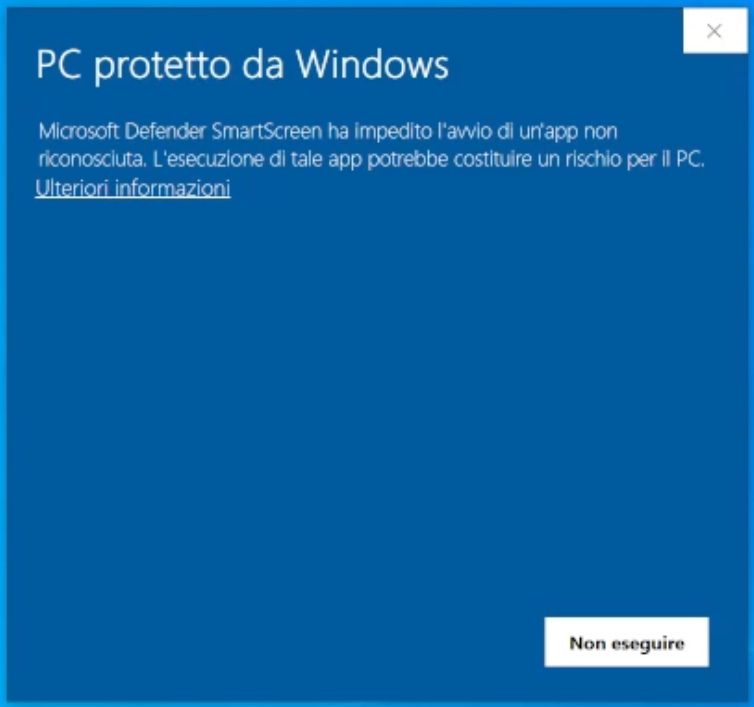
\includegraphics[width=0.5\linewidth]{images/texlive/win/1_smart_screen.png}
    \caption{Avviso di SmartScreen}
    \label{avviso_smart_screen}
\end{figure}
Cliccare "Ulteriori informazioni" per mostrare il pulsante "Esegui comunque" e cliccarlo.
\begin{figure}[H]
    \centering
    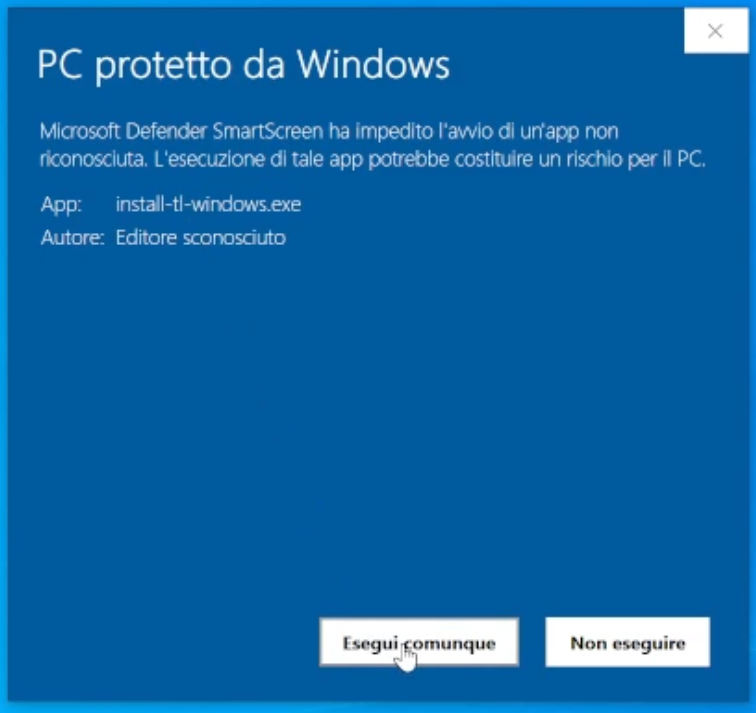
\includegraphics[width=0.5\linewidth]{images/texlive/win/2_smart_screen_2.png}
    \caption{Ulteriori informazioni di SmartScreen}
    \label{info_smart_screen}
\end{figure}
Nella prima schermata dell'installer scegliere "Install", poi premere "Next" e infine "Install".
\begin{figure}[H]
    \begin{subfigure}{0.49\textwidth}
        \centering
        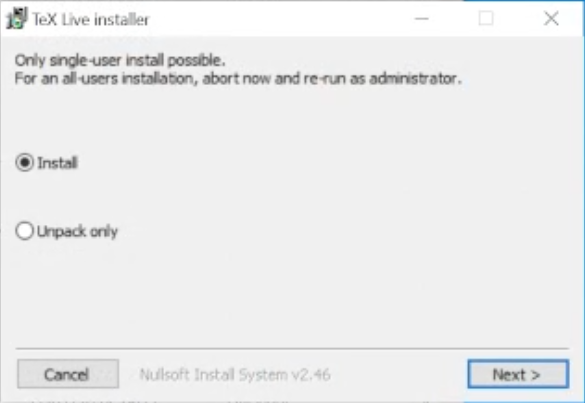
\includegraphics[width=\linewidth]{images/texlive/win/3_install_mode.png}
        \caption{Selezione modalità di installazione}
        \label{texlive_install_mode}
    \end{subfigure}
    \begin{subfigure}{0.49\textwidth}
        \centering
        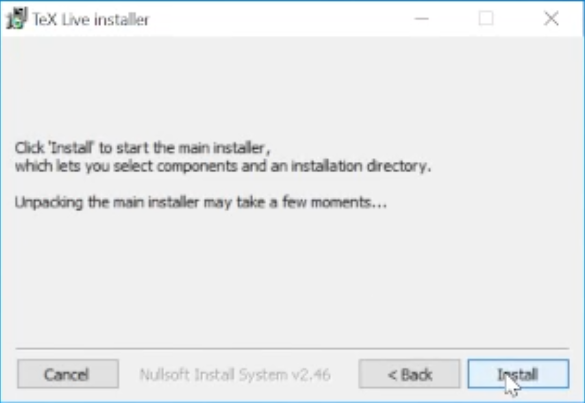
\includegraphics[width=\linewidth]{images/texlive/win/4_start_installer.png}
        \caption{Avvio del configuratore}
        \label{texlive_config}
    \end{subfigure}
\end{figure}
Nella schermata che si apre scegliere il mirror italiano dal menu a tendina.
\begin{figure}[H]
    \centering
    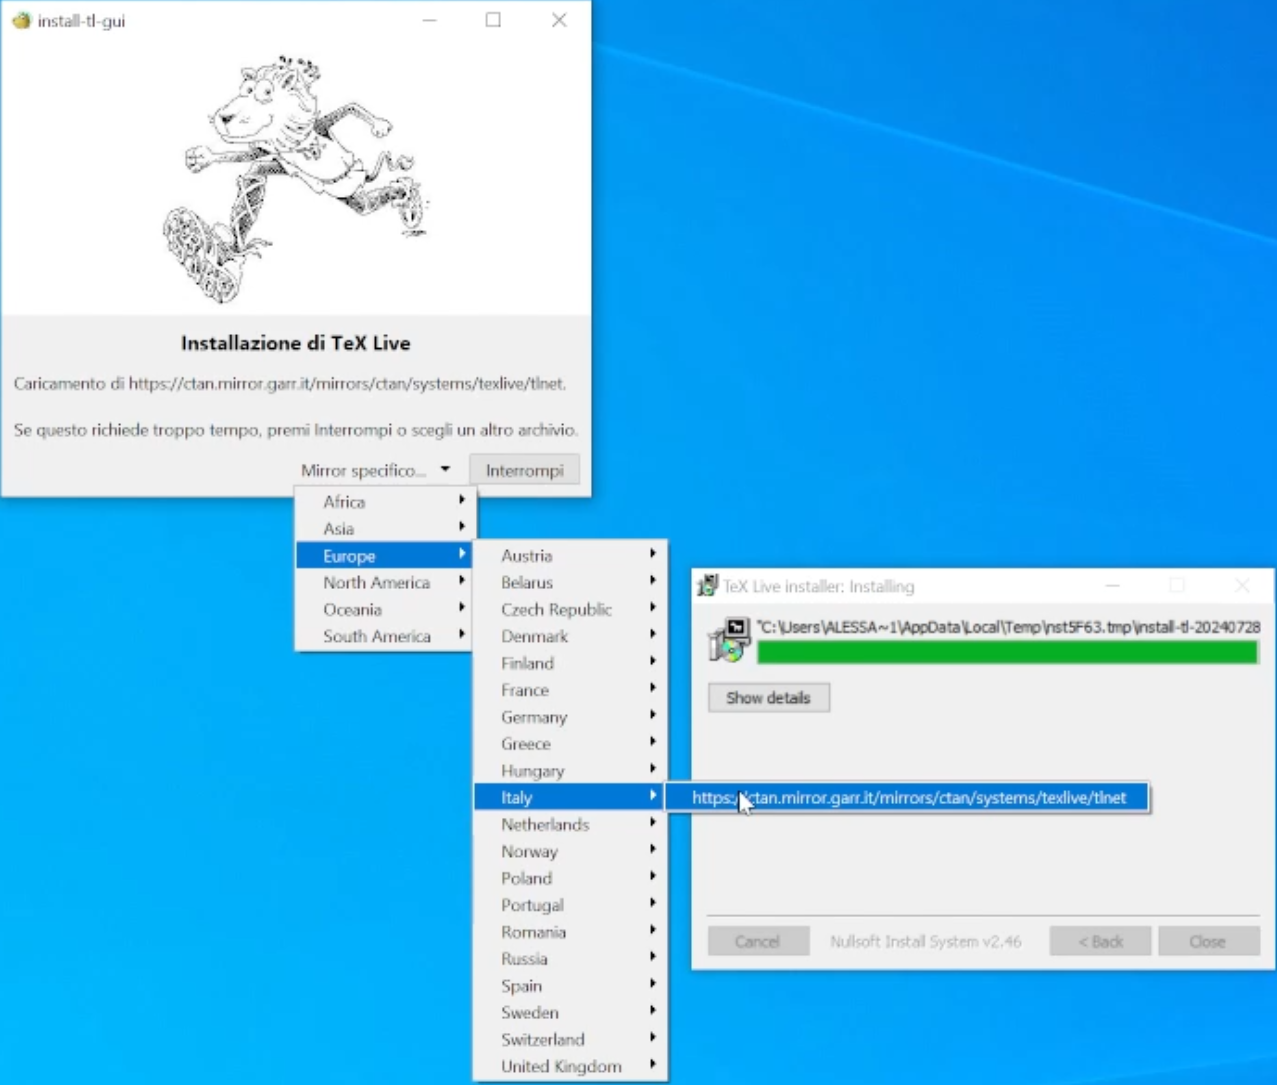
\includegraphics[width=0.95\linewidth]{images/texlive/win/6_mirror_select.png}
    \caption{Selezione del mirror}
    \label{texlive_mirror}
\end{figure}
Dal momento che si userà solo Visual Studio Code per la scrittura, è possibile escludere TeXworks dall'installazione.
Utenti più esperti possono usare le opzioni avanzate per selezionare manualmente i pacchetti da installare
e velocizzare l'installazione. Questa parte non è attualmente oggetto della documentazione e viene lasciata
come triviale esercizio per il lettore.
\begin{figure}[H]
    \centering
    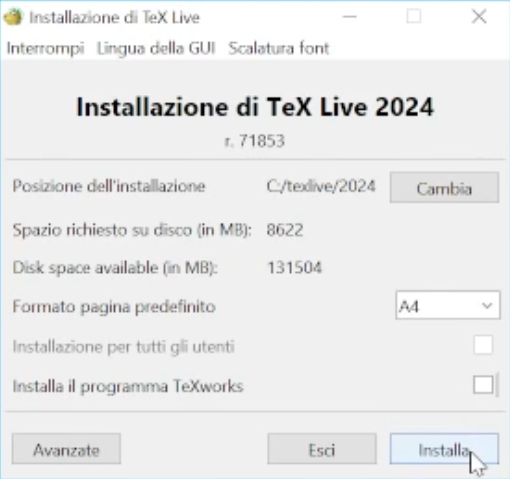
\includegraphics[width=0.8\linewidth]{images/texlive/win/7_configurator.png}
    \caption{Ulteriori configurazioni}
    \label{texlive_config_2}
\end{figure}
L'installazione di tutti i pacchetti può richiedere anche due ore, è possibile continuare a seguire i passaggi successivi di questa guida.
\begin{figure}[H]
    \begin{subfigure}{0.49\textwidth}
        \centering
        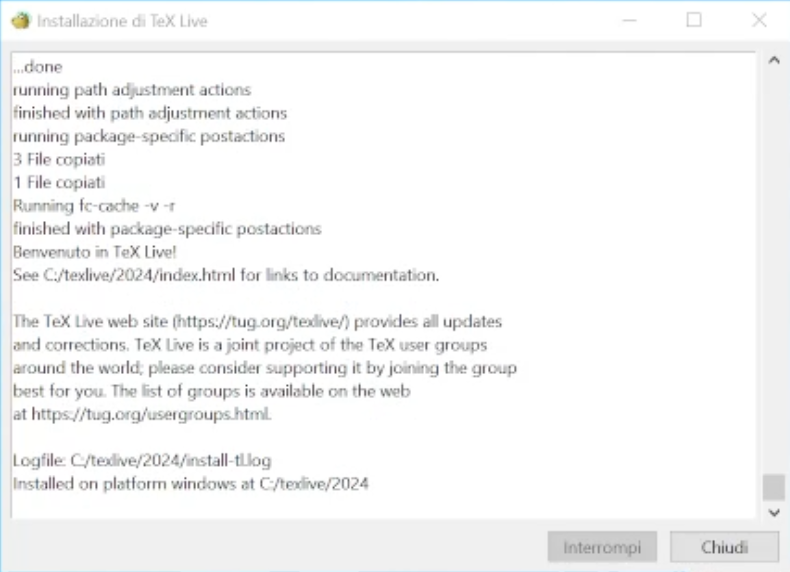
\includegraphics[width=\linewidth]{images/texlive/win/8_download_packages.png}
        \caption{Log di installazione}
        \label{texlive_install_log}
    \end{subfigure}
    \begin{subfigure}{0.49\textwidth}
        \centering
        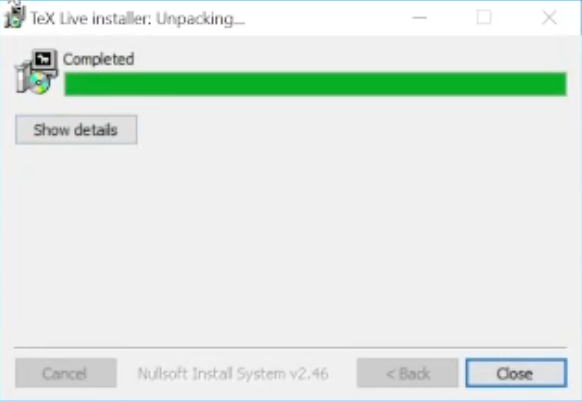
\includegraphics[width=\linewidth]{images/texlive/win/9_end_screen.png}
        \caption{Fine dell'installazione}
        \label{texlive_installato}
    \end{subfigure}
\end{figure}

\label{esempio_citazione}
\subsection{MacOS \citep{installMacTeX}}
Dopo il download di \url{https://mirror.ctan.org/systems/mac/mactex/MacTeX.pkg}, 
fare doppio clic per installarlo. Seguite le semplici istruzioni. 
L'installazione su MacOS recente richiede circa dieci minuti.

Il programma di installazione presenta:
\label{esempio_elenco_numerato}
\begin{enumerate}
    \item una pagina di benvenuto
        \begin{figure}[H]
            \centering
            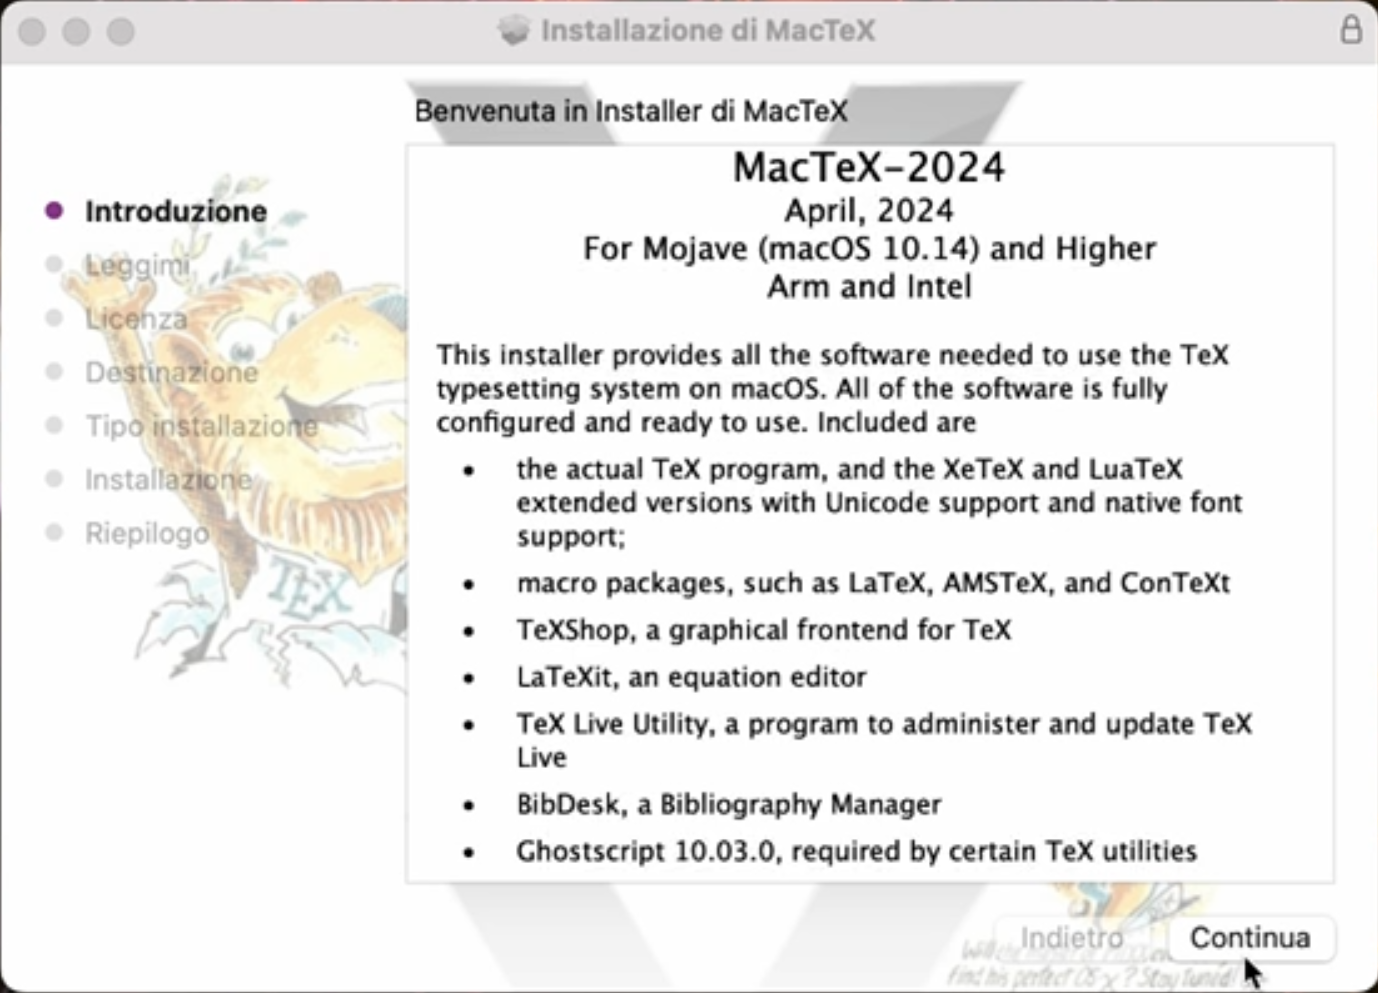
\includegraphics[width=0.5\linewidth]{images/texlive/mac/1_introduzione.png}
            \caption{MacTeX: Introduzione}
            \label{mactex_introduzione}
        \end{figure}
    \item una pagina ReadMe con ulteriori informazioni
        \begin{figure}[H]
            \centering
            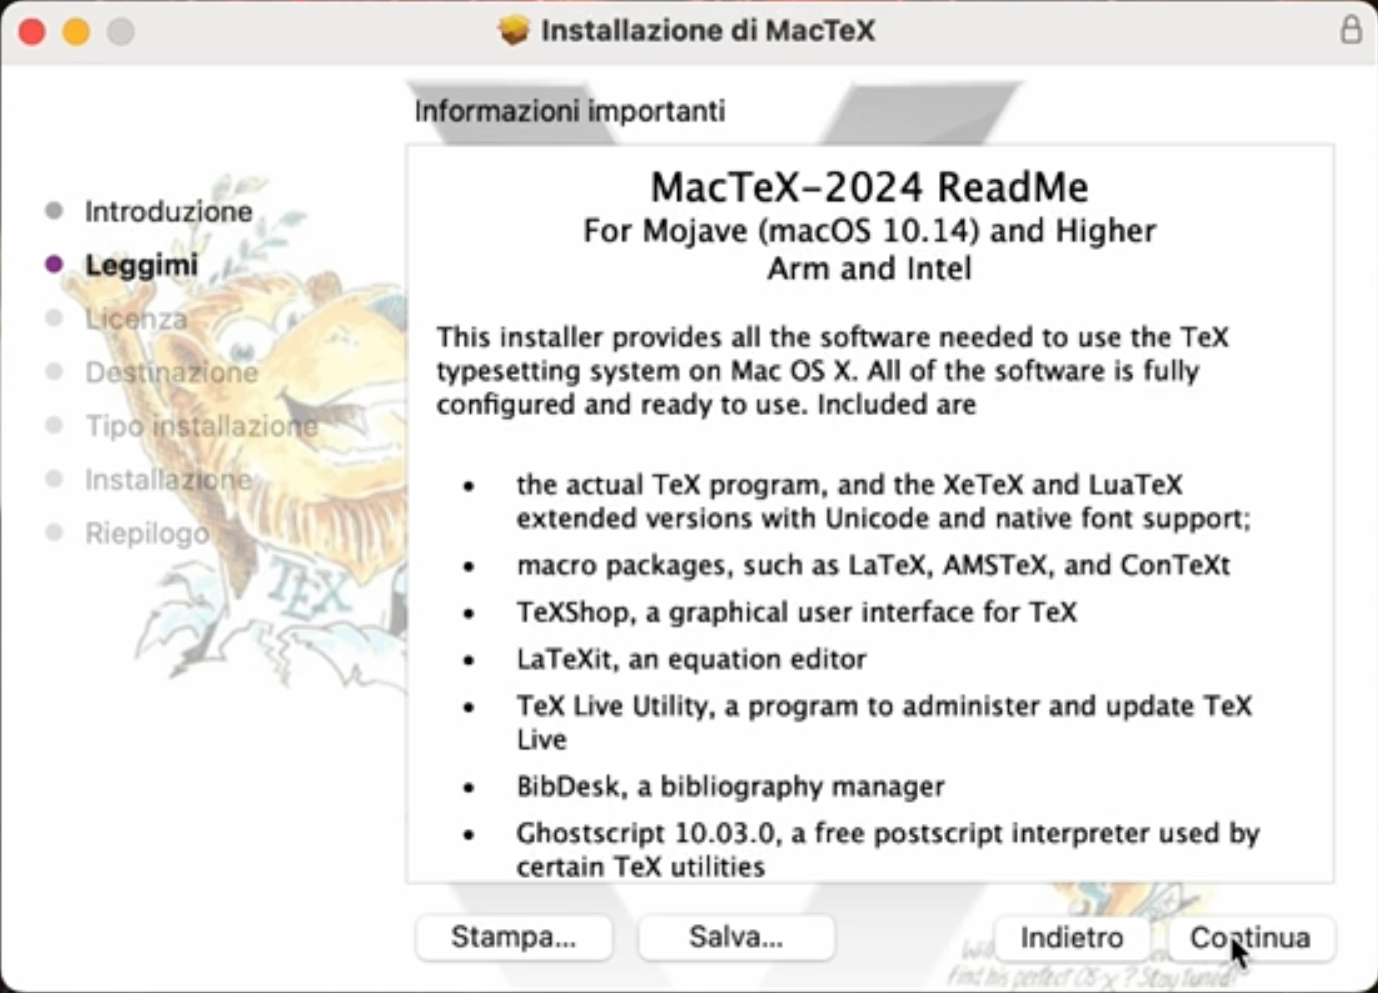
\includegraphics[width=0.5\linewidth]{images/texlive/mac/2_leggimi.png}
            \caption{MacTeX: Leggimi}
            \label{mactex_readme}
        \end{figure}
    \item una pagina di licenza software
        \begin{figure}[H]
            \centering
            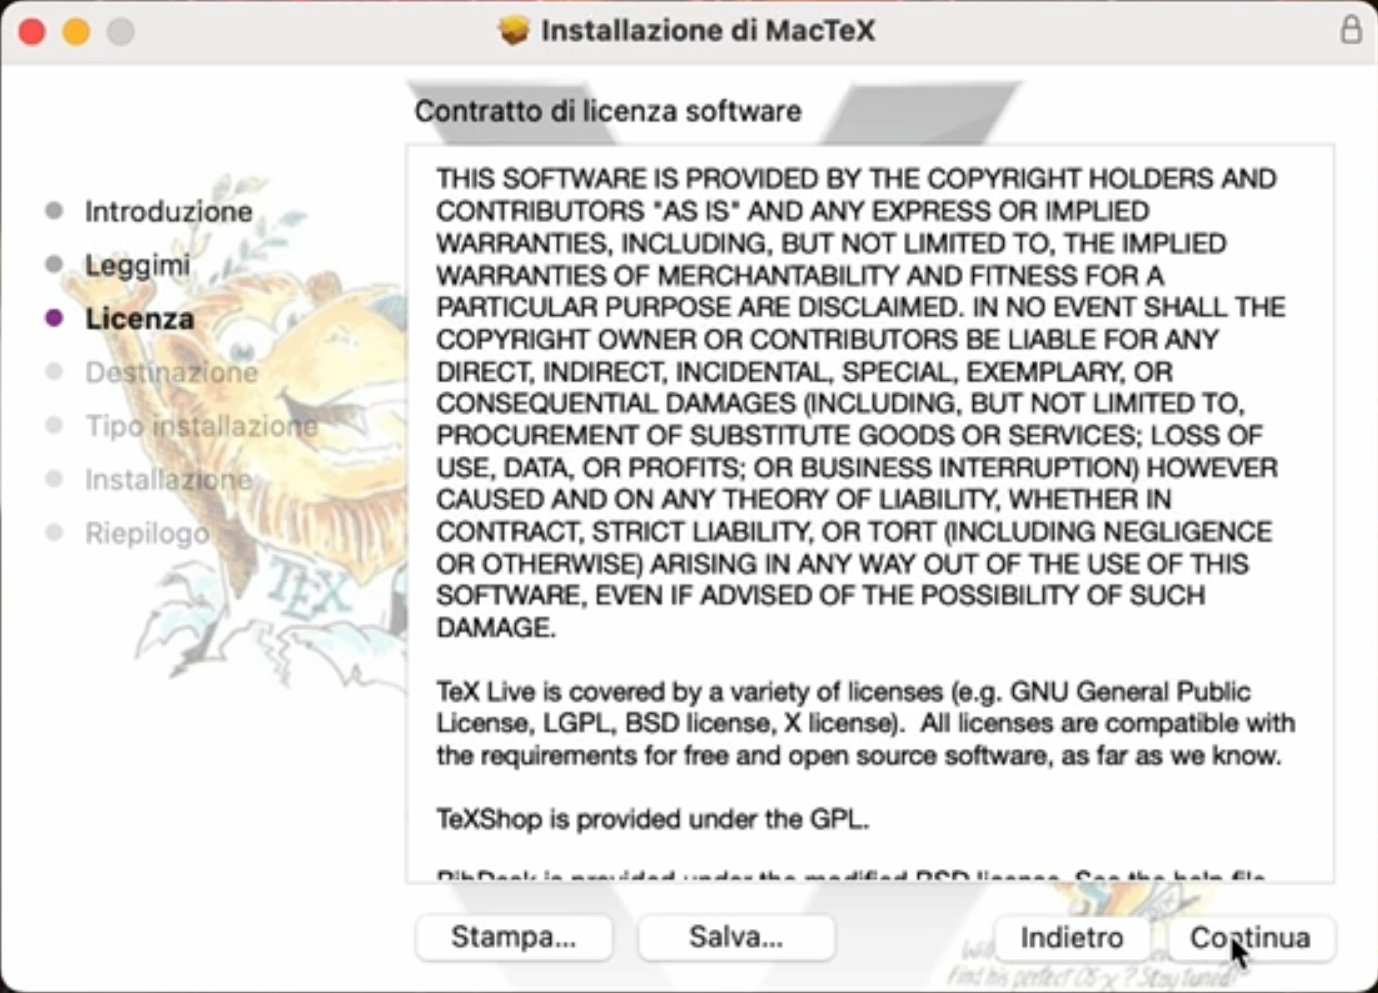
\includegraphics[width=0.5\linewidth]{images/texlive/mac/3_licenza.png}
            \caption{MacTeX: Licenza}
            \label{mactex_licenza}
        \end{figure}
    \item una finestra di dialogo per accettare la licenza
        \begin{figure}[H]
            \centering
            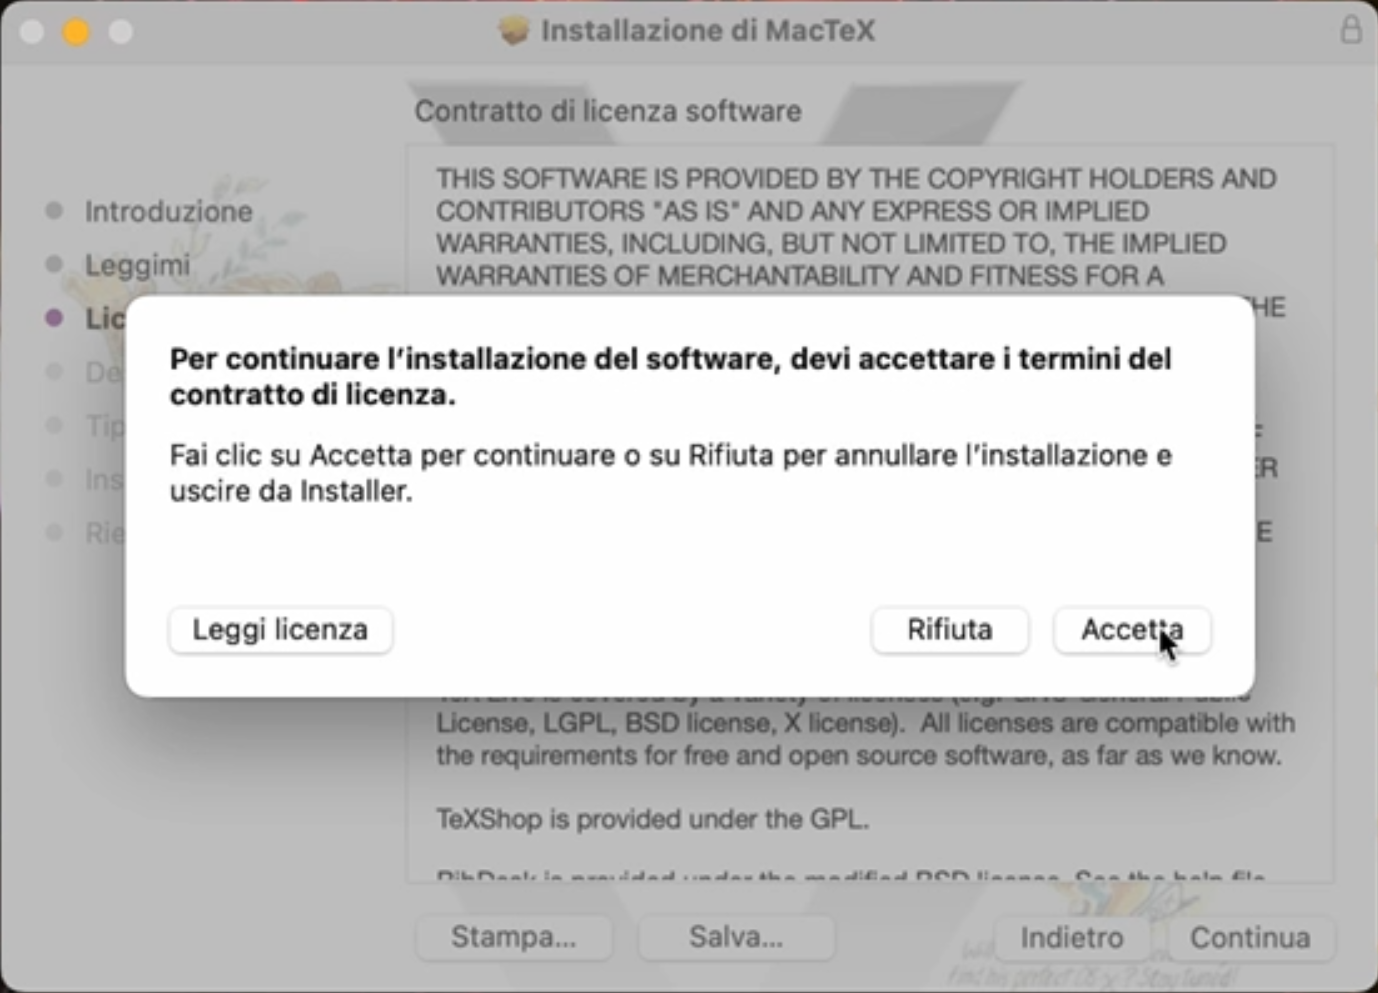
\includegraphics[width=0.5\linewidth]{images/texlive/mac/4_accettazione_licenza.png}
            \caption{MacTeX: Accettazione Licenza}
            \label{mactex_acc_licenza}
        \end{figure}
    \item una pagina di conferma della posizione di installazione
        \begin{figure}[H]
            \centering
            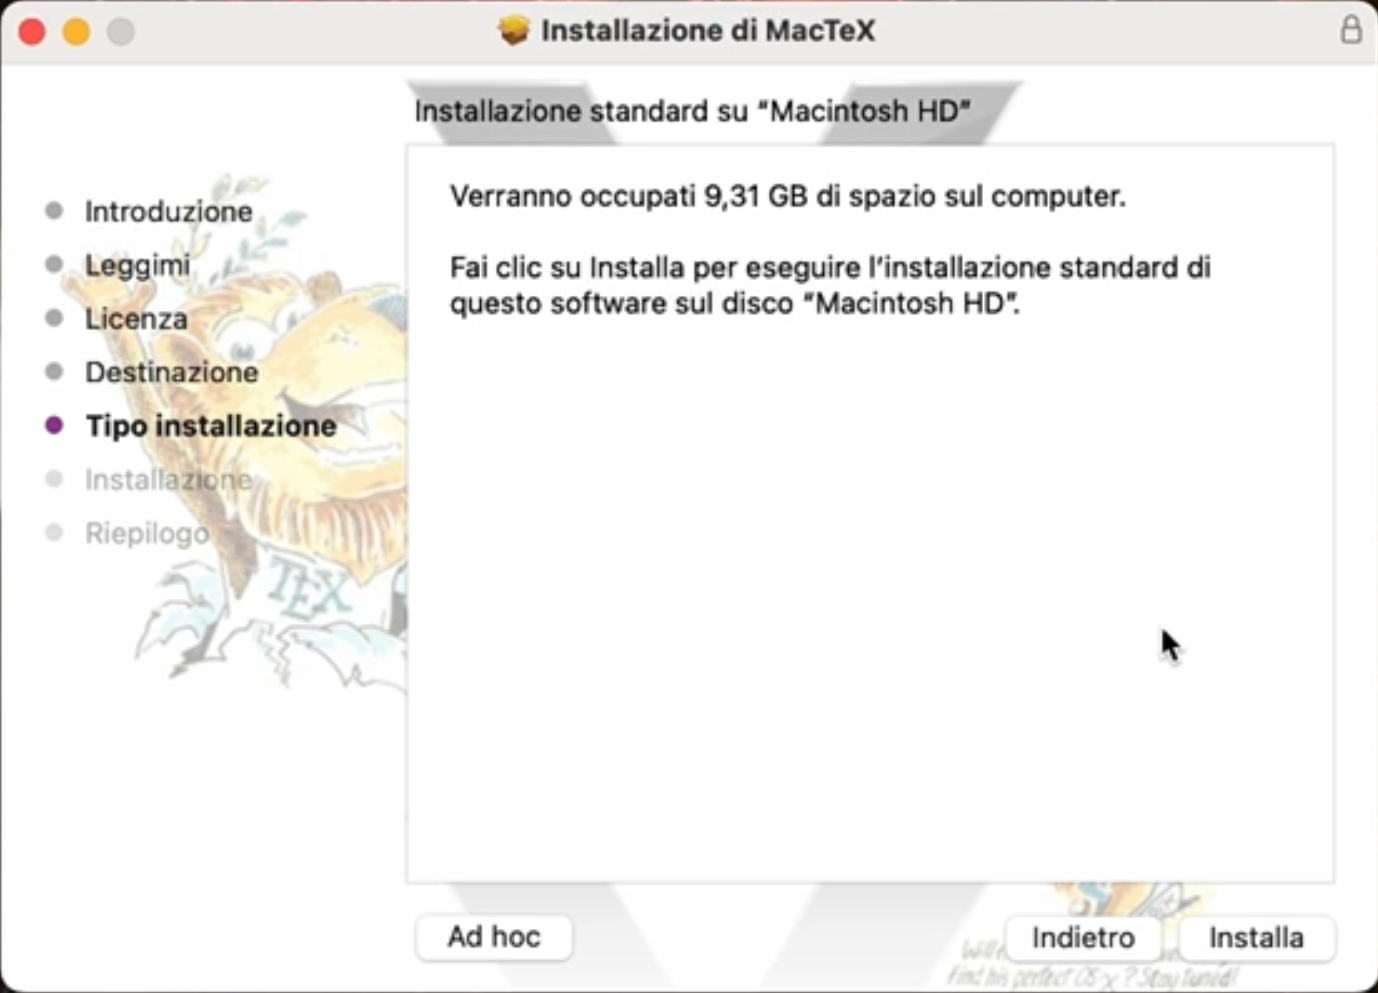
\includegraphics[width=0.5\linewidth]{images/texlive/mac/5_destinazione.png}
            \caption{MacTeX: Destinazione di installazione}
            \label{mactex_dest_installazione}
        \end{figure}
    \item una pagina con il progresso dell'installazione (confermare autenticandosi)
        \begin{figure}[H]
            \centering
            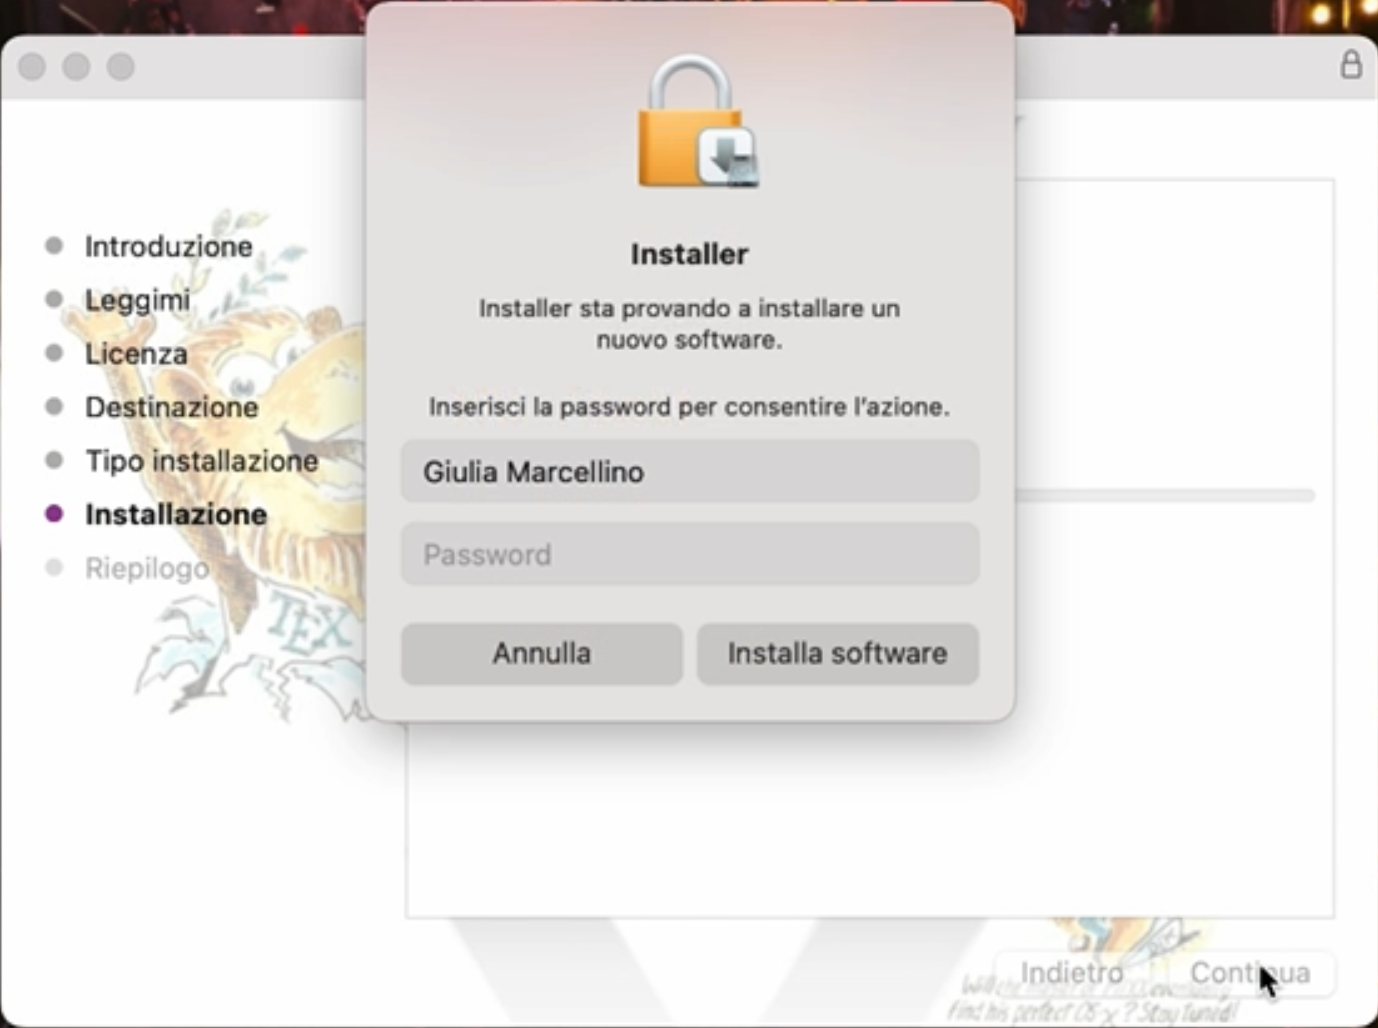
\includegraphics[width=0.5\linewidth]{images/texlive/mac/6_installazione.png}
            \caption{MacTeX: Autenticazione per l'installazione}
            \label{mactex_install_auth}
        \end{figure}
    \item una pagina finale
        \begin{figure}[H]
            \centering
            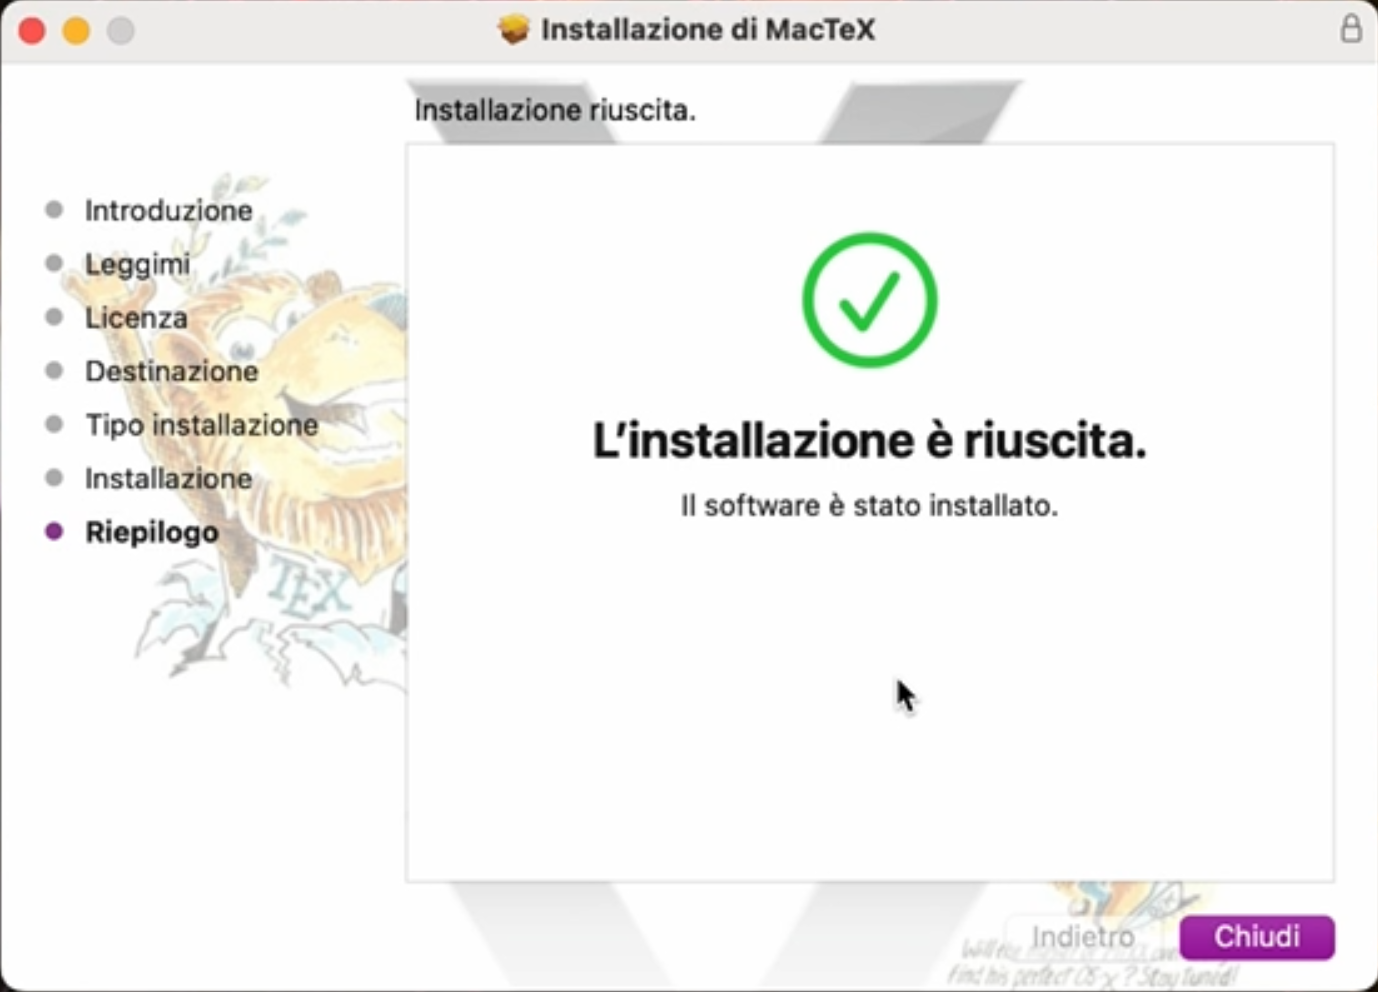
\includegraphics[width=0.5\linewidth]{images/texlive/mac/7_fine_installazione.png}
            \caption{MacTeX: Fine installazione}
            \label{mactex_fine_inst}
        \end{figure}
\end{enumerate}

Al termine dell'installazione una finestra di dialogo chiede se si vuole eliminare l'installer,
spostarlo nel cestino per risparmiare spazio su disco.

\begin{figure}[H]
    \centering
    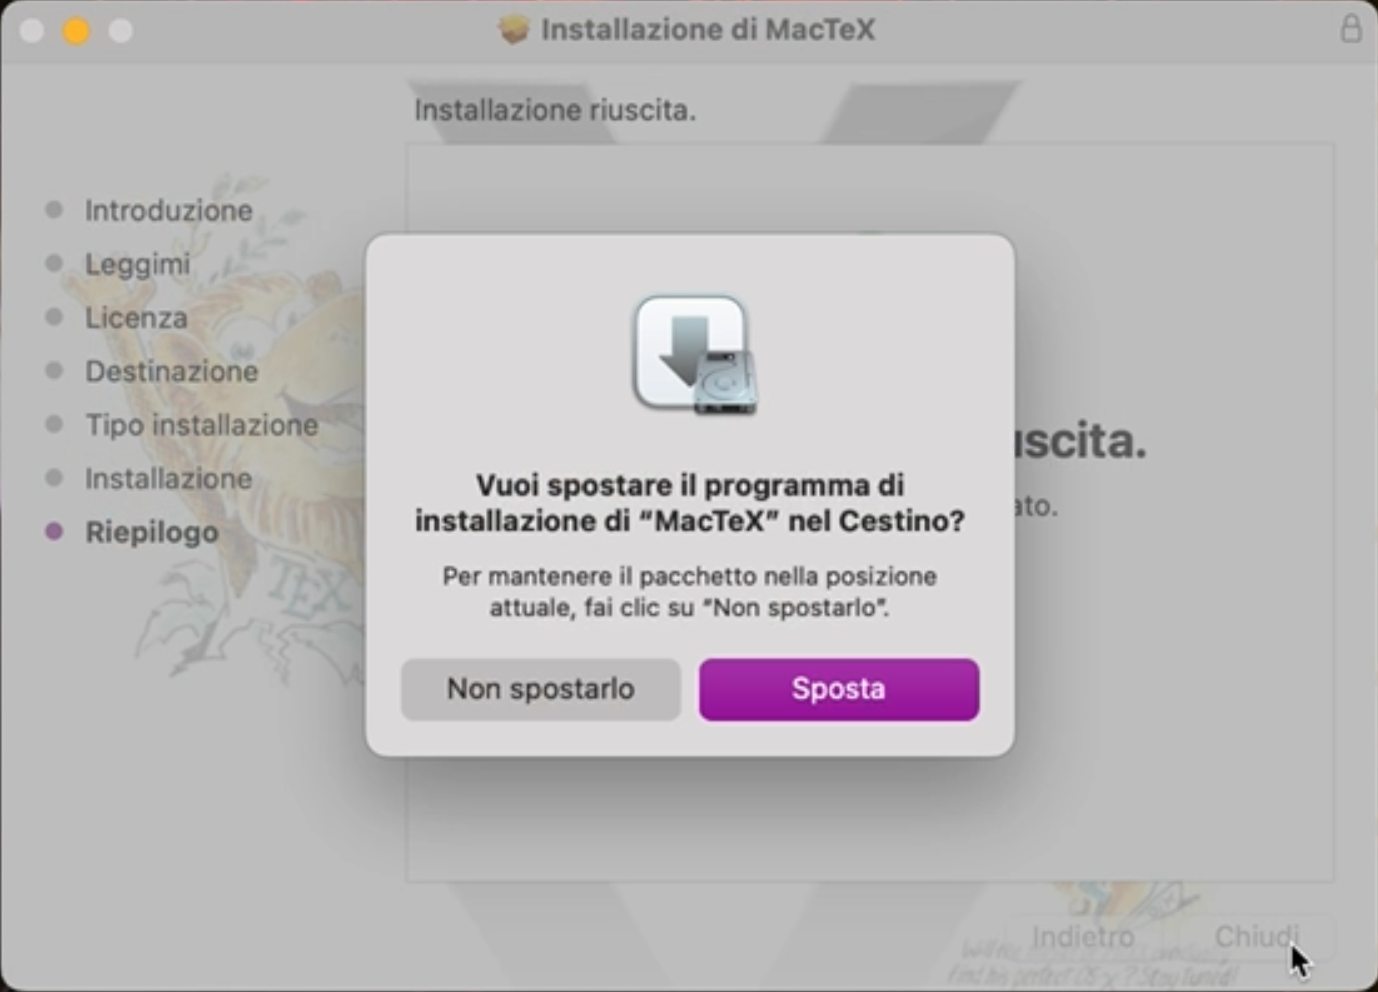
\includegraphics[width=0.9\linewidth]{images/texlive/mac/8_eliminazione_installer.png}
    \caption{MacTeX: Eliminazione installer}
    \label{mactex_eliminazione_installer}
\end{figure}

\subsubsection{Risoluzione dei problemi}\label{sottosottosezione}
\begin{itemize}

    \item \label{enoent} Nel caso in cui la compilazione dei documenti 
        dovesse dare un errore di tipo ENOENT,
        è necessario aggiungere il compilatore al PATH,
        per farlo aprire un terminale e scrivere:
        %gobble rimuove i primi n caratteri dalle righe, permettendo 
        % così di indentare il codice in LaTeX
        %autogobble rimuove automaticamente gli spazi, preservando l'indentazione
        \label{codice_con_minted}
        \begin{minted}[gobble=10]{zsh}
            nano $HOME/.zshrc
        \end{minted}
        Nel file che si apre aggiungere alla fine la riga
        \begin{minted}[gobble=10]{zsh}
            export PATH="/usr/local/texlive/2024/bin/universal-darwin:$PATH"
        \end{minted}
        Per sicurezza verificare il percorso, perchè la cartella {\tt 2024} cambia
         in base alla versione, mentre la cartella {\tt universal-darwin} cambia in base,
         non solo alla versione, ma anche all'architettura del processore.

        Dopo questo passaggio è consigliabile chiudere COMPLETAMENTE Visual Studio Code 
        dal menù in alto a sinistra e riaprirlo, se non dovesse risolvere, 
        riavviare il computer.


    \item A volte, l'installatore visualizza una finestra di dialogo che dice 
        “Verifica...” e poi l'installazione si blocca. In tutti i casi conosciuti, 
        il riavvio del Macintosh risolve il problema. Dopo il riavvio, 
        eseguire nuovamente l'installazione.

    \item Se durante l'installazione vengono segnalati altri problemi, riferirsi alla sezione 
        \href{https://www.tug.org/mactex/mactex-download.html}{“Errori di installazione”} della guida ufficiale.

    \item MacTeX scrive un collegamento simbolico /Library/TeX/texbin che punta 
        alla directory dei binari di TeX Live. Configurare i programmi GUI per utilizzare 
        questo collegamento. I programmi GUI forniti si configurano automaticamente.
    
\end{itemize}


\subsection{Linux e Unix}
Per voi uomini temerari che non avete paura di usare un terminale, 
propongo i comandi per l'installazione su distribuzioni Debian-based:
\begin{minted}{bash}
    sudo apt install texlive-science texlive-latex-extra latexmk \
        texlive-extra-utils texlive-publishers texlive-science
\end{minted}

\section{Visual Studio Code}
Per la scrittura si userà Visual Studio Code, editor multipiattaforma 
estensibile con numerosi plug-in.
D'ora in poi ci si riferirà ad esso col suo nome breve: vscode.

\subsection{Installazione}
\subsubsection{Windows, MacOS e distribuzioni Linux senza snap}
Per l'installazione su queste piattaforme si consiglia di seguire 
direttamente il sito del programma \url{https://code.visualstudio.com/download}.

\subsubsection{Distribuzioni con snap}
\begin{minted}{bash}
    sudo snap install code --classic
\end{minted}

\subsection{Configurazione}
Installato Visual Studio Code e completata la configurazione iniziale (opzionale),
la schermata presentata sarà simile a questa.
\begin{figure}[H]
    \centering
    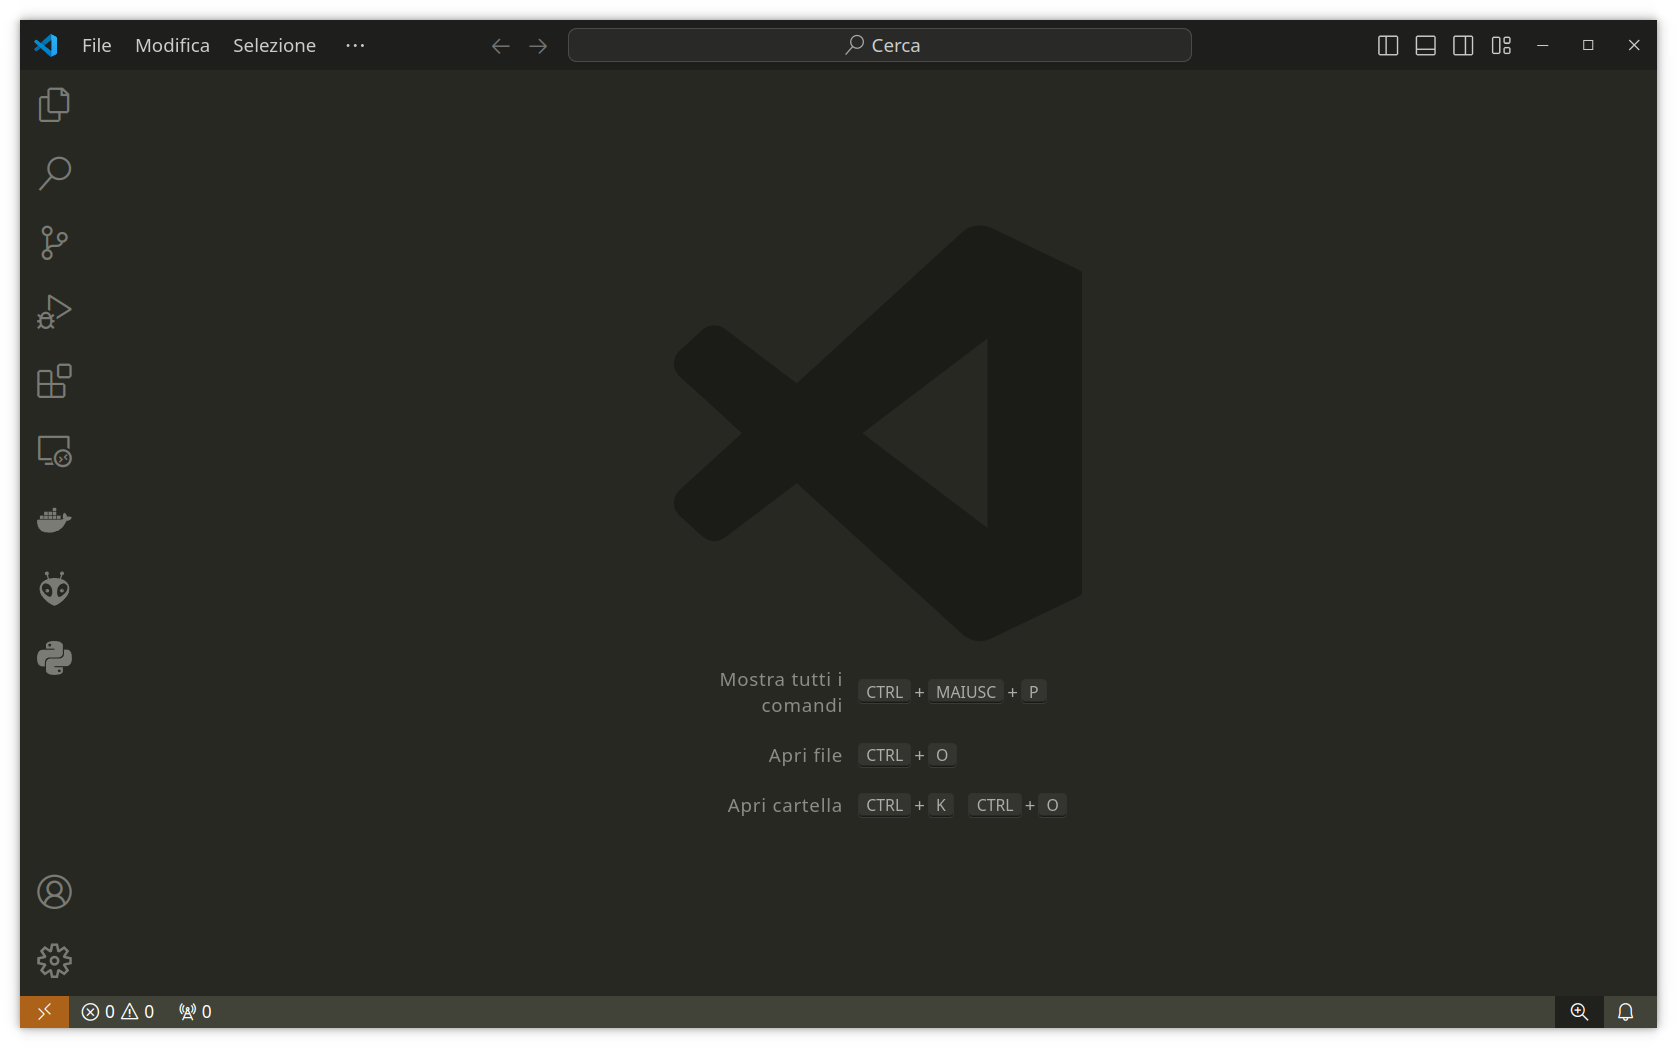
\includegraphics[width=\linewidth]{images/vscode/vscode.png}
    \caption{Schermata iniziale di vscode}
    \label{schermata_iniziale_vscode}
\end{figure}
Cliccare su 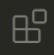
\includegraphics[height=5mm]{images/vscode/estensioni_icona.png}
per aprire il menu delle estensioni.
\begin{figure}[H]
    \centering
    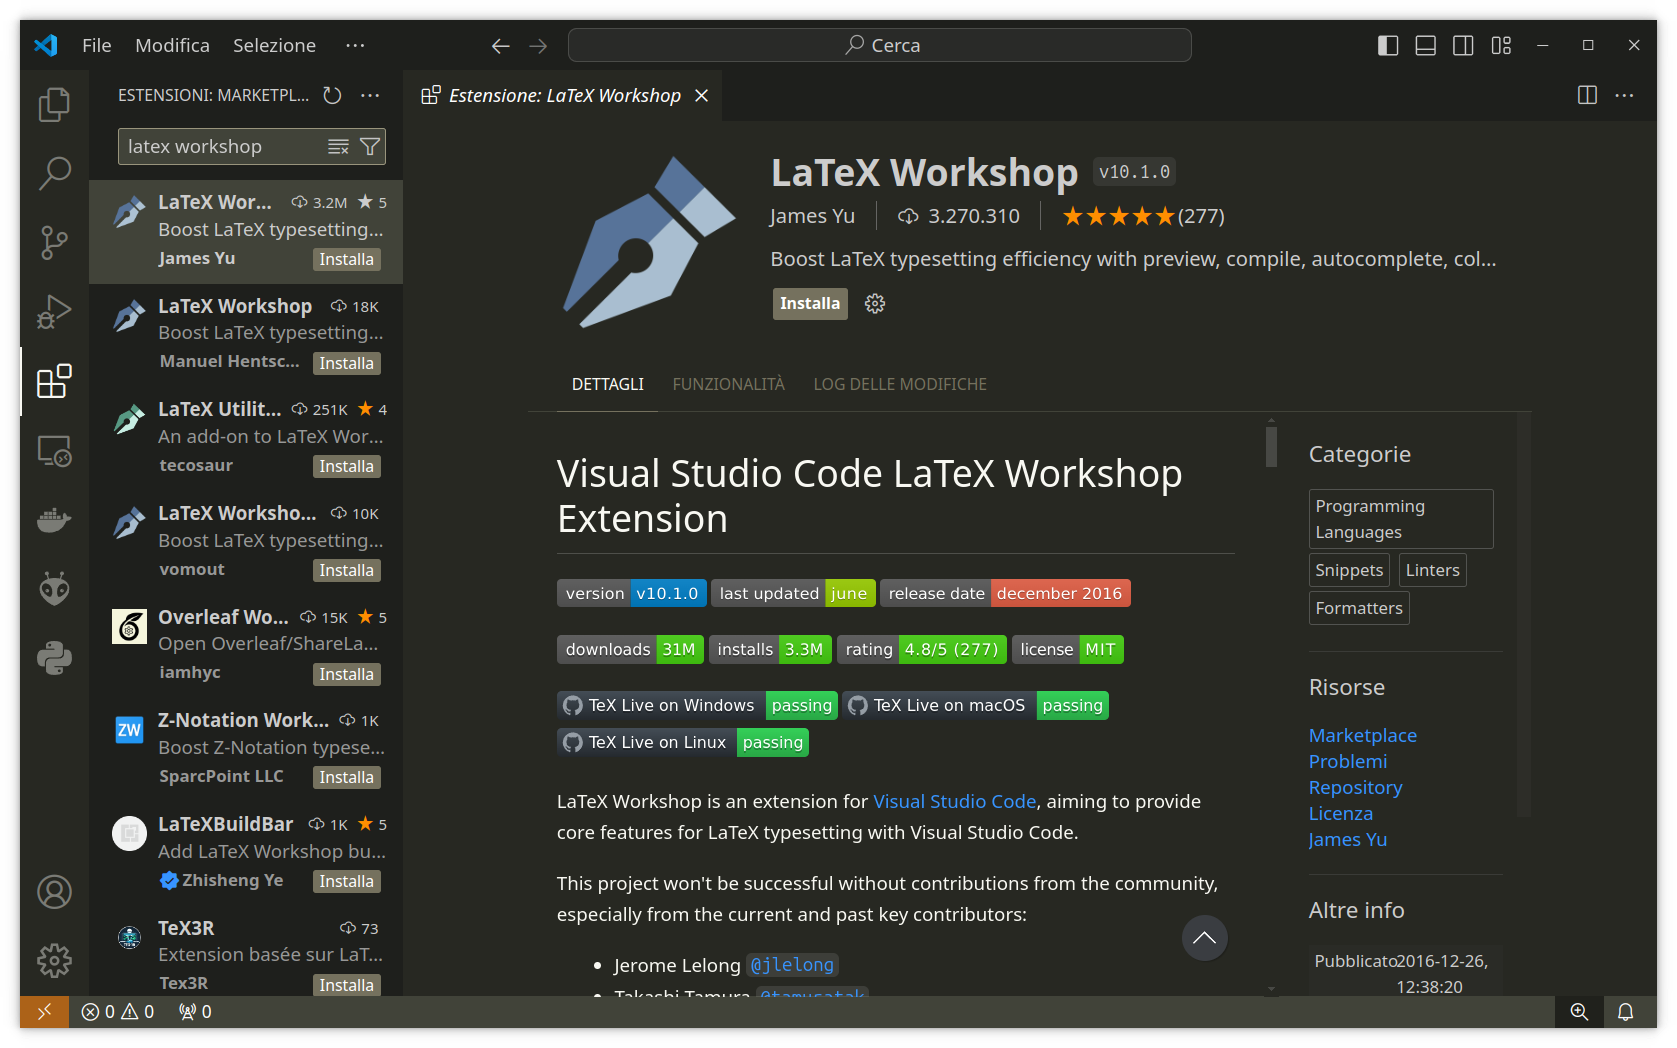
\includegraphics[width=\linewidth]{images/vscode/vscode_latex_workshop.png}
    \caption{Schermata gestore estensioni}
    \label{schermata_gestore_estensioni}
\end{figure}
Nella barra di ricerca cercare Latex Workshop e premere su installa per avviare l'installazione.
Terminata l'installazione aprire il menu delle azioni rapide con Ctrl + Alt + P (Cmd + Alt + P su MacOS).
\begin{figure}[H]
    \centering
    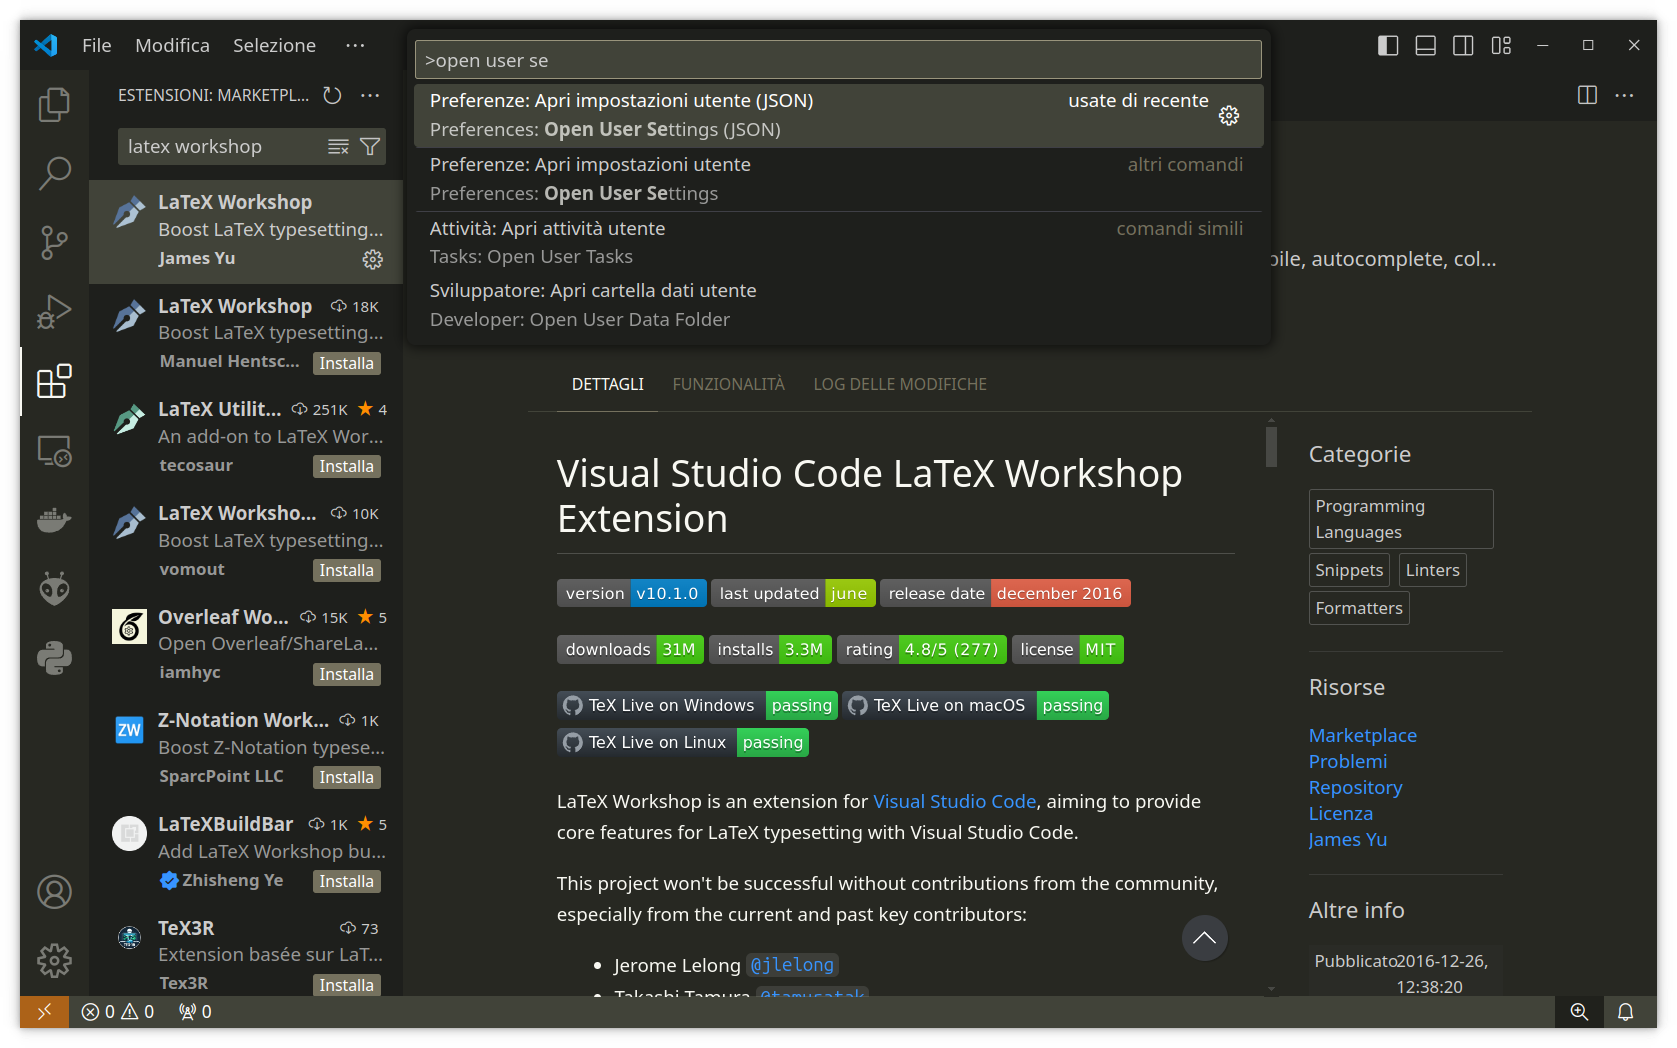
\includegraphics[width=\linewidth]{images/vscode/vscode_user_settings.png}
    \caption{Menu azioni rapide}
    \label{menu_azioni_rapide}
\end{figure}
Cercare "Open User Settings (JSON)" come in figura \ref{menu_azioni_rapide} e selezionare la voce.
\begin{figure}[H]
    \centering
    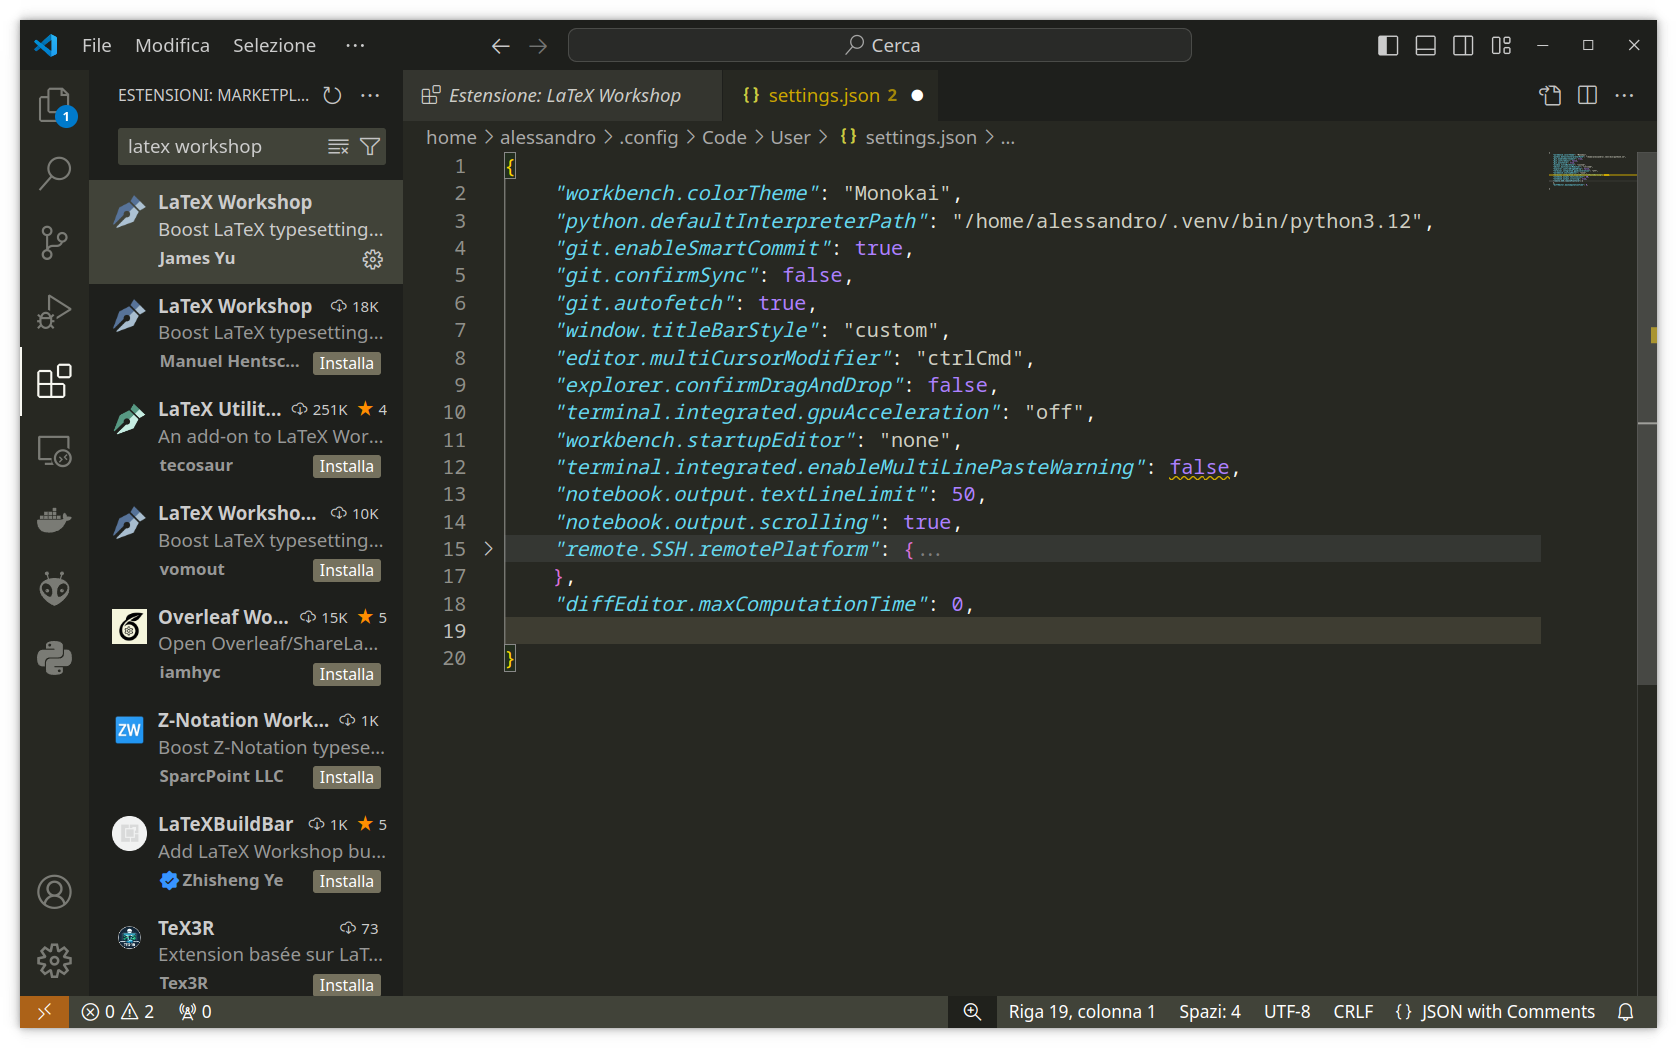
\includegraphics[width=\linewidth]{images/vscode/vscode_settings_json.png}
    \caption{File JSON delle impostazioni}
    \label{json_impostazioni}
\end{figure}
Nella schermata che si apre incollare il contenuto del file 
my\_settings.json presente nella cartella del progetto.
È possibile eliminare il file dopo aver inserito il suo contenuto 
nel file settings.json di vscode.\\
ATTENZIONE: Il file che si sta modificando è un file JSON, in quanto
tale richiede alcuni semplici accorgimenti di sintassi.
Se, come nella figura \ref{json_impostazioni}, sono già presenti altre 
righe, dopo l'ultima è necessario aggiungere una virgola prima 
di incollare il resto delle impostazioni.

Il risultato finale dovrebbe essere qualcosa di simile a \ref{json_impostazioni_nuovo}
\begin{figure}[H]
    \centering
    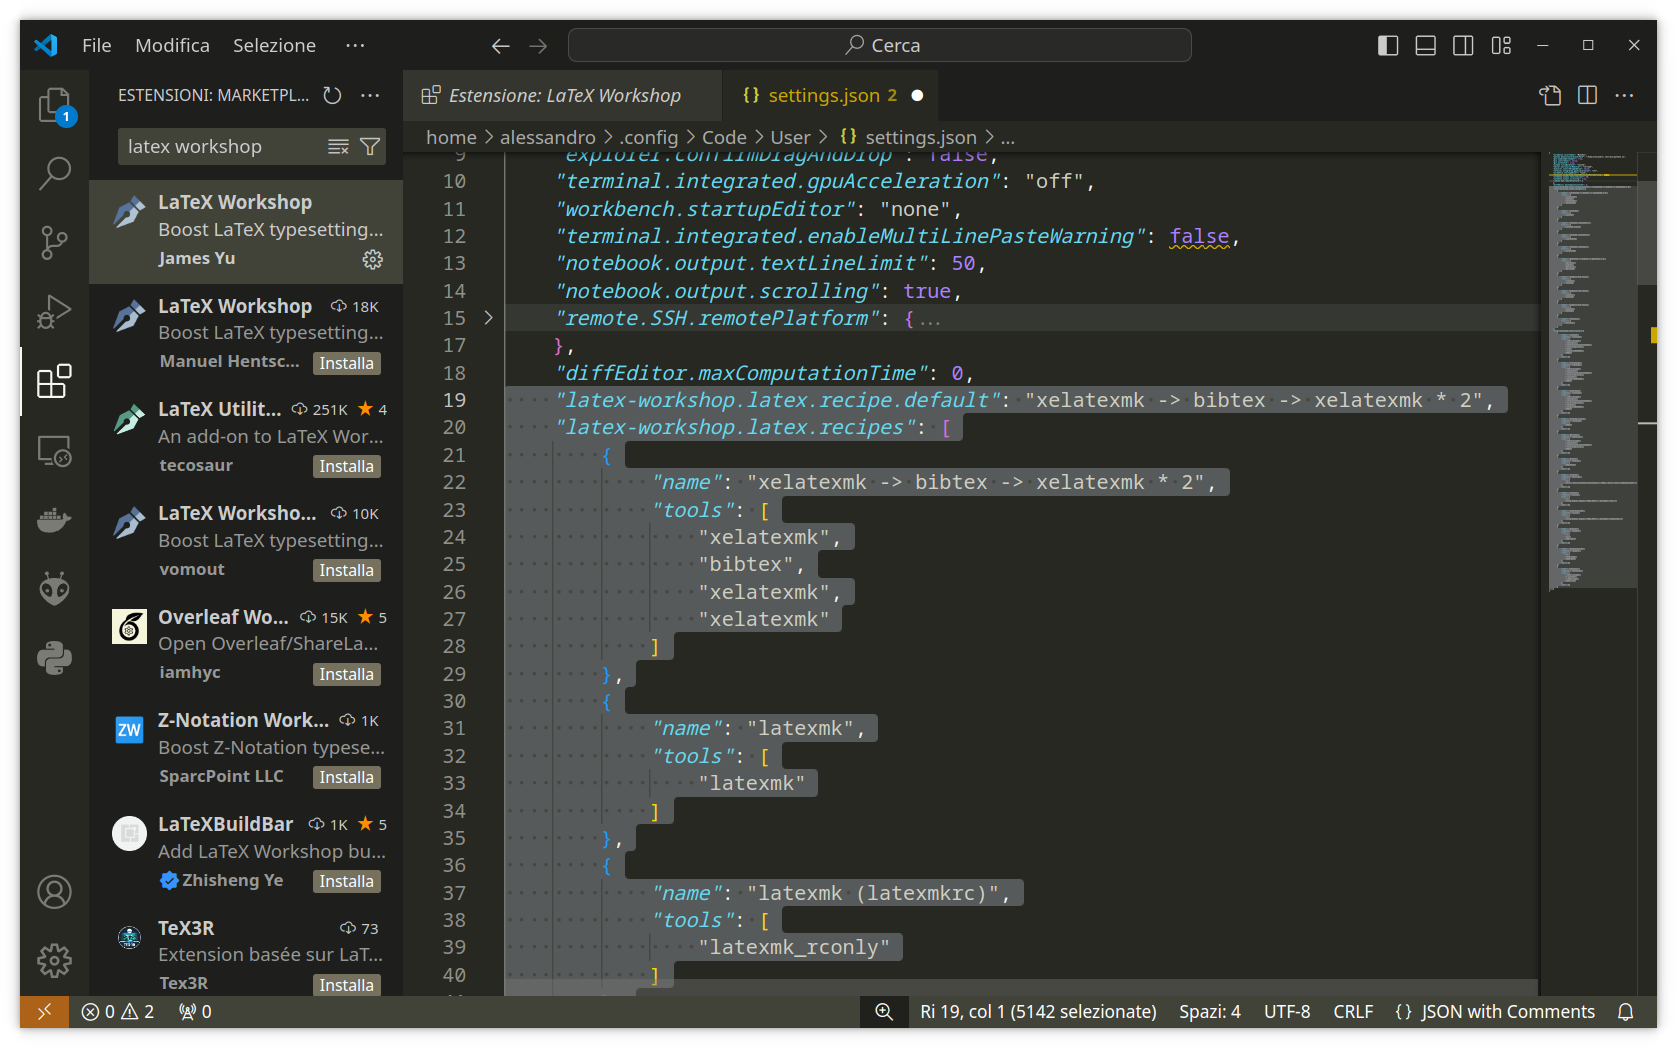
\includegraphics[width=\linewidth]{images/vscode/vscode_settings_json2.png}
    \caption{File JSON delle impostazioni dopo la modifica}
    \label{json_impostazioni_nuovo}
\end{figure}


\chapter{Controllo versione} \label{Cap.2}

\vspace{2cm}

\begin{flushright}
\textit{Breve introduzione al sistema di controllo versione\\ per sincronizzazione dei file del documento su GitHub.}
\end{flushright}

\vspace{0.5cm}

La scrittura di un lavoro di tesi richiede tempo ed è consigliabile che questo 
documento non esista in una sola copia, per evitare disastri e per poter lavorare 
da più dispositivi (se necessario), è altamente consigliabile usare un software
di controllo versione per poter sempre avere traccia delle modifiche e sincronizzarle
con un server remoto all'occorrenza.

Per svolgere questo compito ci si avvarrà del programma git e del servizio GitHub.

\section{Git}
Git è un client che permette la creazione e gestione di repository.
\subsection{Installazione \citep{installGit}}
In base alle prove effettuate, risulta già installato su MacOS, 
quindi questo non verrà documentato.
\subsubsection{Windows}
Cliccando col tasto destro sull'icona di Start, a seconda della versione del 
sistema operativo e della configurazione, cliccare su:
\begin{itemize}
    \item Apri Powershell (Amministratore)
    \item Apri Prompt dei comandi (Amministratore)
    \item Apri Terminale (Amministratore)
\end{itemize}
Nel prompt scrivere {\tt winget install git.git}, accettare con {\tt y} 
e invio quando chiede conferma.

\subsubsection{Linux}
Anche in questo caso l'installazione dipende da distribuzione a distribuzione. 
Per le distribuzioni Debian-based, il comando è il seguente:
\begin{minted}{bash}
    sudo apt install git
\end{minted}

\subsection{Configurazione}
Per poter usare Git è necessario specificare nome e email dell'utente che lo userà.
Sempre nel terminale inserire questi due comandi (validi per tutte le piattaforme)
opportunamente modificati con i vostri dati, è molto importante prestare attenzione
alle virgolette attorno a nome e email:
\begin{minted}{bash}
    git config --global user.name "Mario Rossi"
    git config --global user.email "mario.rossi@unirc.it"
\end{minted}

\section{GitHub}
\label{wrapfigure}
\begin{wrapfigure}{l}{0.10\textwidth}
    \centering
    \vspace{-0.5\linewidth} % Rimuove lo spazio bianco prima della figura
    
\includegraphics[width=\linewidth]{images/github/github.png}
    \vspace{-0.9\linewidth} % Rimuove lo spazio bianco dopo della figura
    %\caption{Logo GitHub}
    \label{logo_github}
\end{wrapfigure}

GitHub è un servizio di hosting per progetti software, che implementa lo strumento 
di controllo versione distribuito Git.
Recandosi alla pagina \url{https://github.com} è possibile registrarsi o accedere al 
proprio account, per poter creare un proprio progetto sulla base di questo modello.

La registrazione è una procedura triviale e non è necessario documentarla.

Recarsi alla pagina \url{https://github.com/a13ssandr0/TesiUnirc} e premere il pulsante 
{\tt Use this template} in alto a destra e poi cliccare su {\tt Create a new repository}.
\begin{figure}[H]
    \centering
    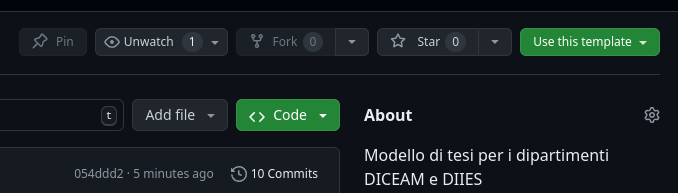
\includegraphics[width=\linewidth]{images/github/template.png}
    \caption{Pulsante creazione da template}
    \label{pulsante_creazione_repository}
\end{figure}

\label{nota_pie_pagina}
Nella pagina che appare dare un nome alla repository\footnote{La 
cartella principale in cui vengono salvati i file.} e concludere con Create repository.
\begin{figure}[H]
    \centering
    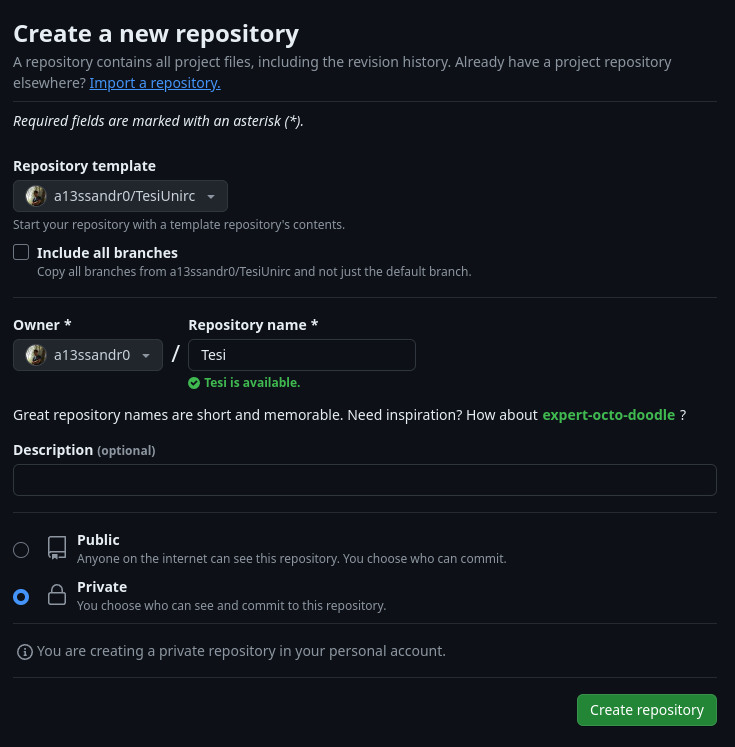
\includegraphics[width=\linewidth]{images/github/new_repo.png}
    \caption{Pagina creazione repository}
    \label{pagina_creazione_repository}
\end{figure}

Terminato il caricamento, GitHub reindirizzerà l'utente alla sua repository, 
la pagina dovrebbe apparire così:

\begin{figure}[H]
    \centering
    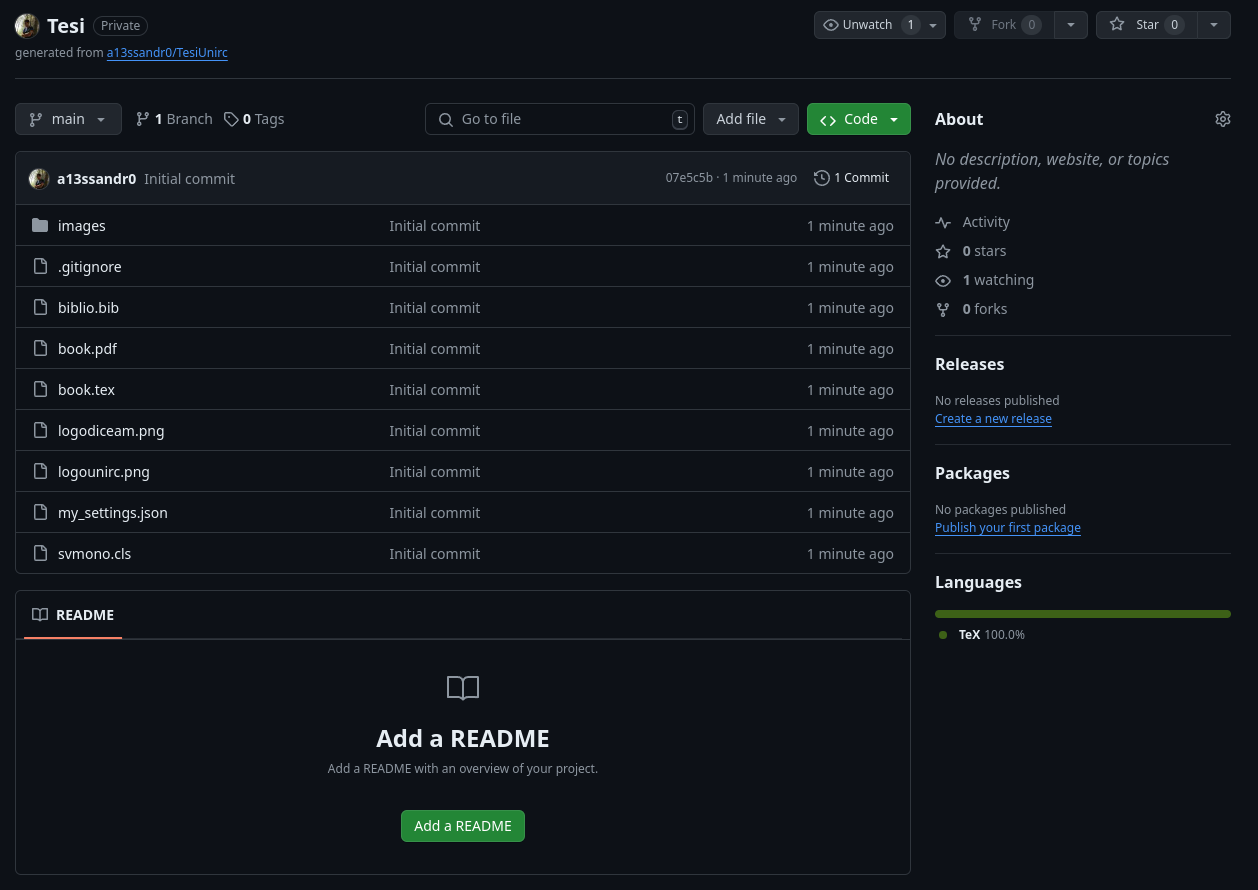
\includegraphics[width=1.5\linewidth]{images/github/new_repo_created.png}
    \caption{Pagina repository}
    \label{pagina_repository}
\end{figure}

\textit{
NOTA: La figura sopra è stata inserita con una larghezza di 1.5 volte la larghezza
standard della colonna di testo, sebbene nel pdf permetta una migliore visualizzazione,
questo espediente è da evitare quando si prepara il documento per la stampa e rilegatura.}

\newpage \label{nuova_pagina}

\section{Visual Studio Code}
Creata la repository personale, è possibile clonarla in vscode. \citep{vscodeGit}
\begin{figure}[H]
    \centering
    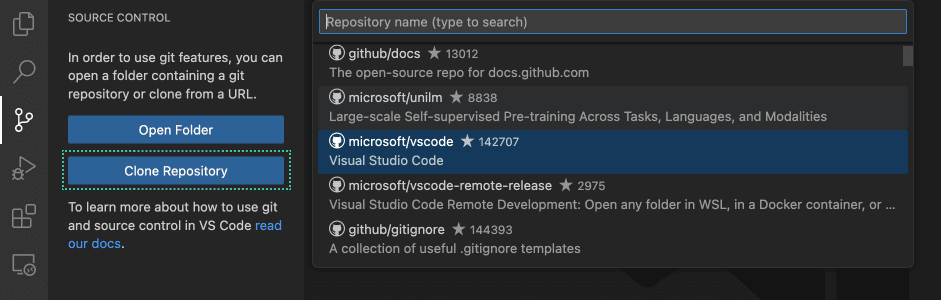
\includegraphics[width=\linewidth]{images/vscode/vscode_clone_repo.png}
    \caption{Menu clonazione repository}
    \label{clonazione_repository}
\end{figure}
La prima volta, prima di far selezionare la repository chiederà di accedere con il 
proprio account GitHub. Inserire il nome della propria repository per clonarla, 
premere invio e selezionare la cartella in cui clonarla.
Vscode automaticamente la scaricherà e aprirà il progetto.

Se tutto è stato configurato correttamente, aprendo il file book.tex comparirà un 
triangolo verde in alto a destra per compilare il documento e creare il pdf, in generale 
il progetto viene ricompilato automaticamente ad ogni salvataggio del file.

Su MacOS è molto probabile che all'esecuzione del compilatore venga restituito un 
errore ENOENT, fare riferimento al primo punto della sezione Risoluzione dei problemi
a pagina \pageref{enoent}.



\chapter{Esempi}  \label{Cap.3}

\vspace{2cm}

\begin{flushright}
 \textit{Altri esempi di scrittura in \LaTeX\\ che non è stato possibile inserire nei capitoli precedenti.}
\end{flushright}

\vspace{0.5cm}

La seguente tabella\footnote{Altri esempi e stili \url{https://www.overleaf.com/learn/latex/Tables}} raccoglie i riferimenti ad elementi usati nelle pagine precedenti.

\begin{table}[h!]
    \centering
    \begin{tabular}{||c | c | c||} 
        \hline
        Sezione & Elemento & Pagina \\ [0.5ex] 
        \hline\hline
        \ref{acronimi} & Indice degli acronimi & \pageref{acronimi} \\ 
        \ref{introduzione} & Capitolo senza numero & \pageref{introduzione} \\
        \ref{esempio_elenco_puntato} & Elenco puntato & \pageref{esempio_elenco_puntato} \\
        \ref{esempio_elenco_puntato} & Elenco numerato & \pageref{esempio_elenco_puntato} \\
        \ref{Cap.1} & Capitolo con numero & \pageref{Cap.1} \\
        \ref{esempio_url} & URL & \pageref{esempio_url} \\
        \ref{sezione} & Sezione & \pageref{sezione} \\
        \ref{sottosezione} & Sottosezione & \pageref{sottosezione} \\
        \ref{sottosottosezione} & Sotto-sottosezione\footnote{Non ti sono bastati 3 livelli? \href{https://tex.stackexchange.com/questions/60209/how-to-add-an-extra-level-of-sections-with-headings-below-subsubsection}{Questo è un link per stackexchange, spiega come aggiungere altri livelli di sottosezioni.}} & \pageref{sottosottosezione} \\
        \ref{codice_con_minted} & Sezioni di codice\footnote{Minted mette a disposizione altri stili oltre a quello prefefinito, riferirsi a \url{https://www.overleaf.com/learn/latex/Code_Highlighting_with_minted}} & \pageref{codice_con_minted} \\
        \ref{wrapfigure} & Figura affiancata al testo & \pageref{wrapfigure} \\
        \ref{nota_pie_pagina} & Nota a piè di pagina & \pageref{nota_pie_pagina} \\
        \ref{nuova_pagina} & Citazione & \pageref{nuova_pagina} \\ [1ex] 
        \hline
    \end{tabular}
    \caption{Questa è una tabella.}
    \label{tabella_esempi}
\end{table}

\section{minted}
Uso del pacchetto {\tt minted} per la visualizzazione di codice Python:
\begin{minted}{python}
import numpy as np
    
def incmatrix(genl1,genl2):
    m = len(genl1)
    n = len(genl2)
    M = None #to become the incidence matrix
    VT = np.zeros((n*m,1), int)  #dummy variable
    
    #compute the bitwise xor matrix
    M1 = bitxormatrix(genl1)
    M2 = np.triu(bitxormatrix(genl2),1) 

    for i in range(m-1):
        for j in range(i+1, m):
            [r,c] = np.where(M2 == M1[i,j])
            for k in range(len(r)):
                VT[(i)*n + r[k]] = 1;
                VT[(i)*n + c[k]] = 1;
                VT[(j)*n + r[k]] = 1;
                VT[(j)*n + c[k]] = 1;
                
                if M is None:
                    M = np.copy(VT)
                else:
                    M = np.concatenate((M, VT), 1)
                
                VT = np.zeros((n*m,1), int)
    
    return M
\end{minted}


\section{Testo multicolonna}

\begin{multicols}{2}
    \textbf{Colonna 1}\\
    Testo della prima colonna.\\
    Lorem ipsum dolor sit amet, consectetuer adipiscing elit. Etiam lobortis facilisis sem.
    \columnbreak\\
    \textbf{Colonna 2}\\
    Testo della seconda colonna.\\
    Lorem ipsum dolor sit amet, consectetuer adipiscing elit. Etiam lobortis facilisis sem. Nullam nec mi et neque pharetra sollicitudin. Praesent imperdiet mi nec ante. Donec ullamcorper, felis non sodales commodo, lectus velit ultrices augue, a dignissim nibh lectus placerat pede.
\end{multicols}

\newpage
\section{Spazi e ritorni}
{\tt \textbackslash newpage} termina la pagina attuale e inizia una nuova pagina.

Segue uno spazio vuoto di 2cm.

\vspace*{2cm}

Per forzare uno o più spazi bisogna usare uno o più backslash, ognuno seguito da uno spazio.\\
Testo normale\\
Testo \ con uno spazio in più\\
Testo \ \ con due spazi in più\\
Testo \ \ \ con tre spazi in più\\

Per forzare \LaTeX\ ad inserire una nuova riga vuota, inserire uno spazio e poi andare a capo.\\
\begin{verbatim}
\ \\
\end{verbatim}
Per scrivere questa sezione è stato usato il blocco {\tt verbatim}, il testo al suo interno non viene
interpretato in alcun modo.



Un elenco di elenchi??

Roba degna del più famoso elencatore d'Italia. \citep{elencatoreSeriale}
\begin{itemize}
    \item Dell'aria
    \item Dell'acqua
    \item Dei fiumi
    \item Dei mari
    \item dei nostri boschi
    \item delle nostre montagne
    \item dei nostri ghiacciai
    \begin{itemize}
        \item puliti
        \item riciclabili
        \item rinnovabili
        \item biodegradabili
    \end{itemize} 
\end{itemize}





\newpage
\begin{landscape}
    \section{Testo orizzontale}
    landscape ruota il contenuto della pagina in orizzontale.
    
    Per scrivere un'equazione su \LaTeX si può ricorrere a molteplici modi:
    \begin{itemize}
        \item $F=ma$
        \item Per centrare l'equazione:
        \[E=mc^2\]
    \end{itemize}
    Se si vuole numerare e centrare l'equazione si procede in questo modo:
    \begin{equation}
        F=ma 
    \end{equation}

\end{landscape}
    


\chapter*{Conclusioni}
\addcontentsline{toc}{chapter}{Conclusioni}
\markboth{Conclusioni}{Conclusioni}

\vspace{2cm}

\begin{flushright}
 \textit{<SINTESI DELLE CONCLUSIONI>}
\end{flushright}

\vspace{0.5cm}

Le conclusioni funzionano come tutti gli altri capitroli.

Come l'introduzione questo capitolo non ha il numero.

\section*{Sezione delle conclusioni}
La sezione con l'asterisco non ha il numero.

\chapter*{Ringraziamenti}
\addcontentsline{toc}{chapter}{Ringraziamenti}
\markboth{Ringraziamenti}{Ringraziamenti}

\sout{Ringrazio il dipartimento DIIES per aver pubblicato un modello di tesi non troppo aggiornato.}

Ringrazio Alessandro\footnote{``ringrazio me stesso" è poco radiofonico.}
per aver aggiornato il modello e aver scritto la documentazione
per installare tutti i programmi per lavorare al documento.

Ringrazio Gemma e Gabriele per aver fornito parte degli esempi presenti in queste pagine.

Ringrazio Giulia per aver fornito le immagini dell'installazione su MacOS.




\bibliographystyle{apalike}
\bibliography{biblio}

\end{document} 